%%%%%%%%%%%%%%%%%%%%%%%%%%%%%%%%%%%%%%%%%%%%%%%%%%%%%%%%%%%%%%%%%%%%%%%%%%%%%

\chapter{Contexte historique}

\section{La musique en Russie au début du XIX\ieme{} siècle}

Au début du XIX\ieme{} siècle, la Russie accuse un retard considérable pour ce qui est de la musique instrumentale (symphonies, concertos, etc..). Les compositeurs sont étrangers et se produissent essentiellement à Saint-Pétersbourg. C'est également une période où le pays se transforme profondément. La société devient plus citadine et pratique davantage la musique occidentale.

En 1802, la \emph{société philharmonique de Saint-Pétersbourg} est créée par des personnalités du monde de la culture, du monde de la finance, de riches aristocrates et des musiciens. La capitale découvre les œuvres peu connues de Haydn, Mozart et Beethoven. À titre d'exemple, la \emph{Missa Solemnis} de Beethoven y est créée le 26 mars 1824, soit deux semaines avant la première viennoise.

Malgré les guerres napoléoniennes, la culture et la musique française demeurent très appréciées par la haute société. Il en est de même pour l'opéra italien. Rossini est découvert au cours des années 1820 et Verdi au cours des années 1840. Des musiciens tels que John Field (professeur de Mikhaïl Glinka) ou encore Anton Herke (professeur de Piotr Tchaïkovski et Modeste Moussorgski) se chargeront de diffuser l'œuvres des romantiques occidentaux. A partir des années 1830, la russie reçoit des personnalités telles que Liszt (1836), les époux Schumann (1844), Berlioz (1847), etc\dots

\section{La naissance de la musique russe}

À partir de 1783, Saint-Pétersbourg se dote d'un opéra : le \emph{Théâtre de Pierre}. Celui-ci sera modernisé en 1802, 1818 et 1836. Comme la vie musicale s'intensifie, trois autres établissements sont érigés : le \emph{Théâtre Alexandrinski} (1832), le \emph{Théâtre Mikhailovski} (1833) et le très célèbre \emph{Théâtre Mariinski} (1833).

Mais c'est avec les compositeurs Mikhaïl Glinka (1804-1857) et Alexandre Dargomyjski (1813-1869) que la Russie engage une nouvelle direction avec le développement d'une musique prétendue authentiquement russe. Pour la première fois, il est fait emploi de matériaux historiques et traditionnels d'un façon réaliste. Le critique musical moderne Viktor Korchikov résume ainsi la situation :\\
« \emph{On ne peut pas imaginer le développement de la culture musicale russe sans [\dots] les trois opéras : \emph{Ivan Soussanine} (Glinka, 1836), \emph{Rouslan et Ludmila} (Glinka, 1837-1842) et \emph{Le Convive de pierre} (Dargomyjski, 1866-1869)} ».

Un autre tournant consiste en la création, en 1858, de la \emph{Société Musicale Russe}. Sous l'impulsion d'Anton Rubinstein et sous le patronage de la grande-duchesse Elena Pavlovna, cette société a pour mission de répandre l'enseignement de la musique classique et contemporaine au sein de l'empire. La \emph{Société Musicale Russe} gagne très rapidement en professionnalisme. Avec le soutien du prince Nikolaï Troubetskoï, Nicolaï Rubinstein (le frère de d'Anton Rubinstein et grand ami de Piotr Tchaïkovski) devient président de la \emph{Société Musicale de Moscou}. La fondation des conservatoires de Saint-Pétersbourg (1862) puis de Moscou (1866) compte parmi les plus grandes réussites. Très rapidement, la \emph{Société Musicale Russe} s'installe à Kiev (1861), à Kazan (1864), à Kharkov (1871), à Nijni Novgorod (1873?), etc\dots{} La révolution de 1917 marque la dissolution d'une cinquantaine d'antennes disséminées dans tout l'empire. 

\section{Le Groupe des Cinq}

Les guerres napoléoniennes ont entrainé une prise de conscience nationale et l’émergence d'un patriotisme officialisé sous le règne de Nicolas I\ier{} (1825-1855).  Sous Alexandre II (1855-1881) puis Alexandre III (1881-1894), les conditions plus libérales sont optimales pour le développement de la \emph{Société Musicale Russe} et du fameux \emph{Groupe des Cinq}.

Le \emph{Groupe des Cinq} est un cercle de musiciens plus ou moins autodidactes fédérés à partir de 1857 par Mili Balakirev (chef d'orchestre empirique, 1837-1910). César Cui (ingénieur en fortifications, 1835-1918) et Modeste Moussorgski (officier, 1839-1881) furent les premiers à rejoindre le groupe, suivis par Nicolaï Rimski-Korsakov (élève officier de marine, 1844-1908) en 1861 et Alexandre Borodine (médecin et chimiste, 1833-1887) en 1862.

Le groupe défend l'idéal d'une musique authentiquement russe (folklore national, orientalisme), libérée de la tutelle des écoles italienne ou allemande. Il est réfractaire au cosmopolitisme des frères Rubinstein mais promeut la musique romantique moderne (Berlioz, Chopin, Liszt, Schumann) plus novatrice et peu encore diffusée en Russie. En 1868, Piotr Tchaïkovski, qui entretient de bonnes relations avec Mili Balakirev et Nicolaï Rimski-Korsakov, espère devenir le sixième membre du groupe. L'éloignement géographique - Tchaïkovski enseigne au conservatoire de Moscou, le \emph{Groupe des Cinq} est basé à Saint-Pétersbourg - et l'ouverture trop européenne de Tchaïkovski interdisent ce rapprochement. À partir de 1872, la réussite et la « traîtrise contrapuntique » de Rimski-Korsakov, l'échec persistant de Cui et la mort de Moussorgski et Borodine ont raison du cénacle.

Le \emph{Groupe des Cinq} laisse une production musicale importante\footnote{\emph{Islamey} et \emph{Tamara} pour Balakirev, \emph{Le Prince Igor} et \emph{Dans les steppes de l'Asie centrale} pour Borodine, \emph{Une nuit sur le mont Chauve}, \emph{Boris Godounov} et \emph{Tableaux d'une exposition} pour Moussorgski, \emph{Shéhérazade}, \emph{Capriccio espagnol} et \emph{Le Coq d'or} pour Rimski-Korsakov, \dots} et jouit d'un rôle de premier ordre dans l'histoire de la musique.

Une dizaine d'années après la dissolution du groupe des \emph{Groupe des Cinq}, Balakirev est directeur de la Chapelle impériale de Saint-Pétersbourg. Avec Rimski-Korsakov est comme assistant, il occupe cette fonction de 1883 à 1894. C'est pendant ces années qu'il reconstitue un second cercle de musiciens\footnote{D'autres groupes ont existé, citons par exemple le \emph{cercle Belaïev} de Saint-Pétersbourg (1885-1908) avec Nikolai Rimski-Korsakov, Alexander Glazunov, Vladimir Stasov, Anatoly Liadov, Alexander Ossovski, Witold Maliszewski, Nikolai Tcherepnin, Nikolay Sokolov, Alexander Winkler, etc\dots} dont le membre le plus éminent n'est autre que Sergueï Liapounov.\\

La figure \ref{frise} récapitule la chronologie des principaux événements depuis la naissance de Mikhaïl Glinka jusqu'à la mort de Sergueï Liapounov.

\begin{figure}[!ht]
  \begin{bigcenter}
    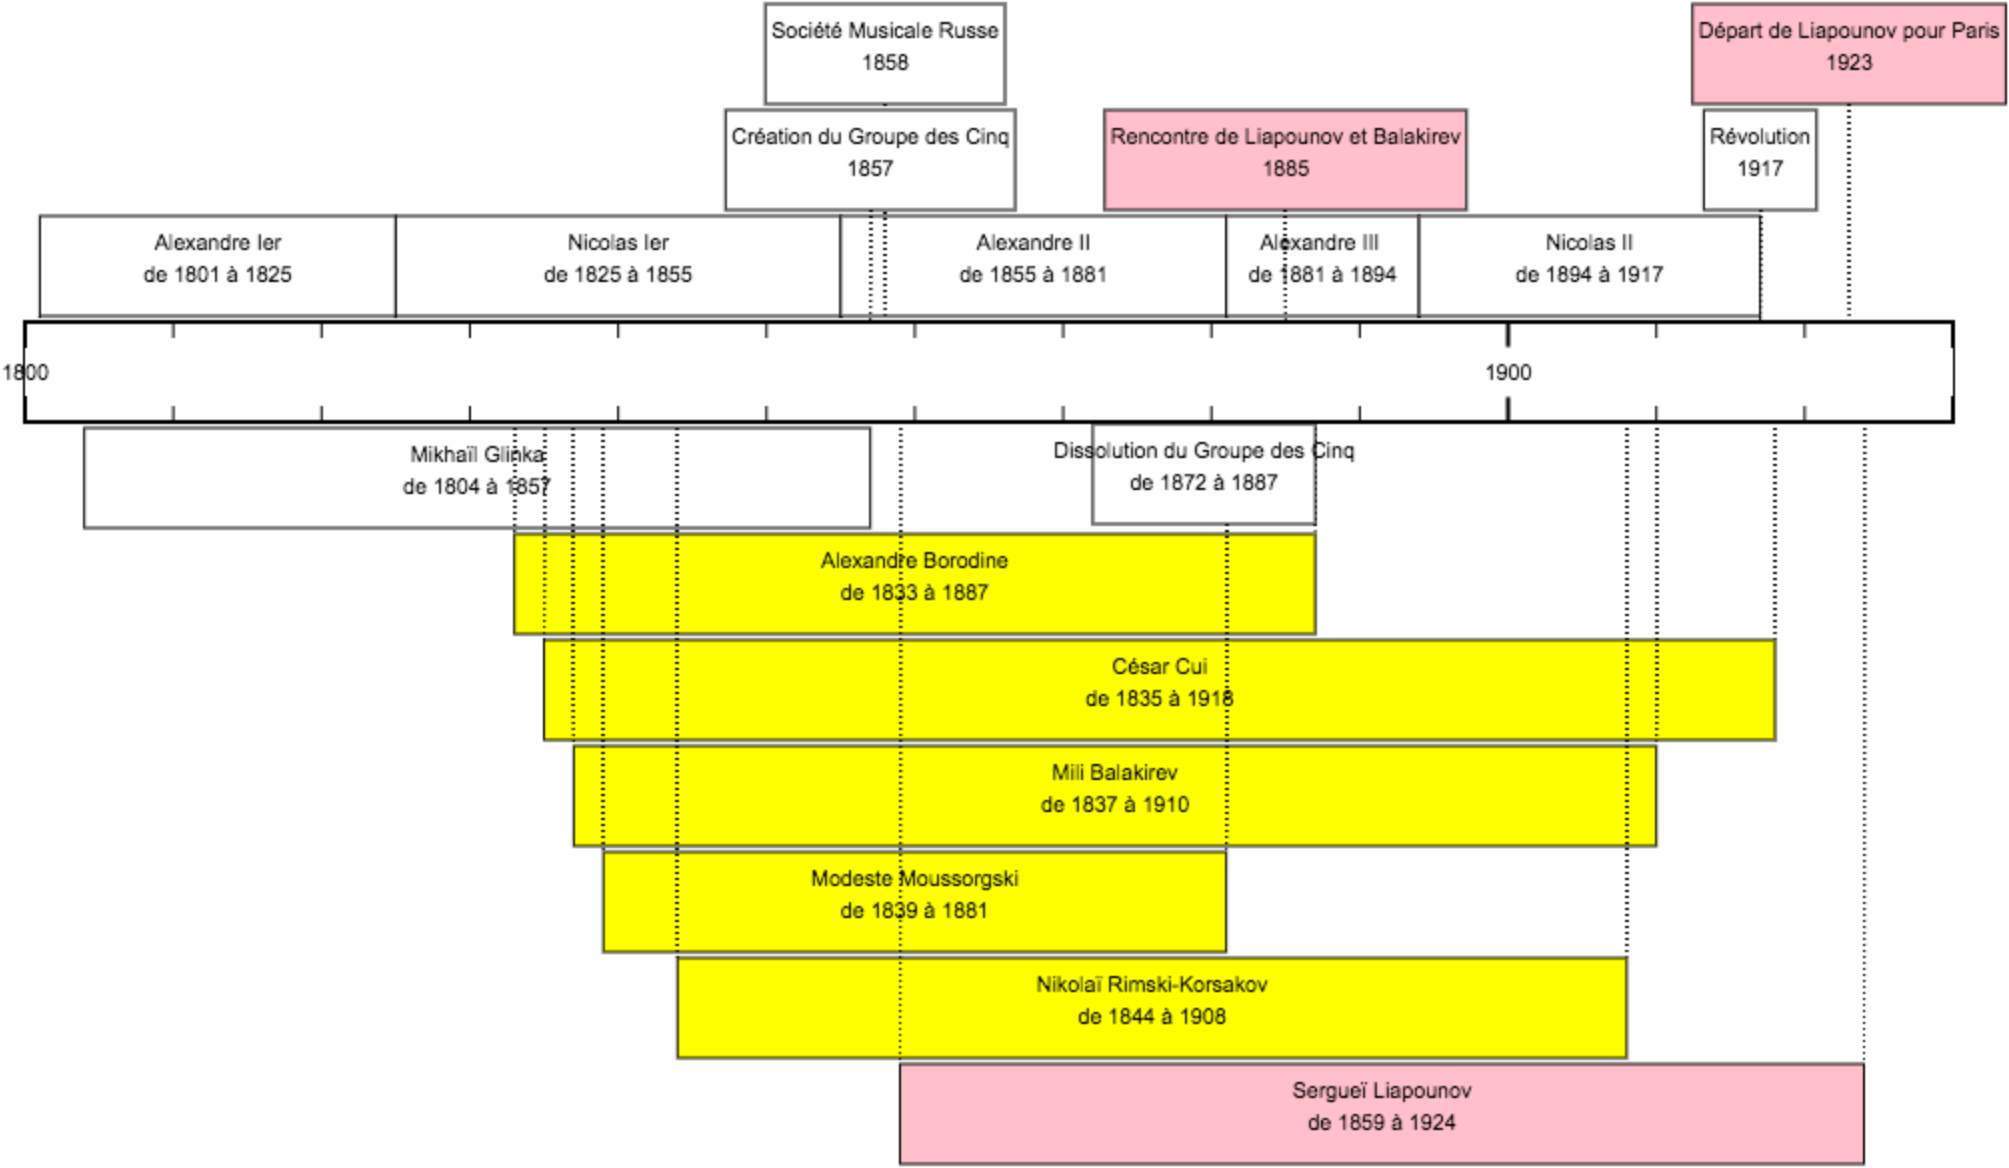
\includegraphics[width=17.5cm, keepaspectratio]{frise.png}
  \end{bigcenter}
  \caption{\label{frise}Frise chronologique des principaux événements depuis la naissance de Mikhaïl Glinka jusqu'à la mort de Sergueï Liapounov.}
\end{figure}

%%%%%%%%%%%%%%%%%%%%%%%%%%%%%%%%%%%%%%%%%%%%%%%%%%%%%%%%%%%%%%%%%%%%%%%%%%%%%

\chapter{L'œuvre de Sergueï Liapounov}

Ce chapitre est dédié à l'étude de la bibliographie et de l'œuvre Sergueï Liapounov.

\section{La jeunesse du compositeur}

Sergueï Mikhaïlovitch Liapounov (\foreignlanguage{russian}{Сергей Михайлович Ляпунов}) est un compositeur, pianiste virtuose, chef d'orchestre, éthnomusicologue, éditeur et pédagogue russe, né le 30 novembre 1859 à Iaroslavl\footnote{Iaroslavl est la capitale administrative de l'oblast de Iaroslavl. La ville est située au confluent de la Volga et de la Kotorosl, à 282 km au nord-est de Moscou.} et mort le 8 novembre 1924 à Paris. Son père, Mikhail Vassilievitch Liapounov, astronome à l'université de Kazan, et sa mère, Sofia Aleksandrovna Shilipova, ont eu trois fils. L'aîné, Alexandre Liapounov (1857-1918), est un célèbre mathématicien connu pour ses travaux sur l'étude des systèmes dynamiques. Le cadet, Boris Liapounov (1862–1943), est un linguiste spécialisé dans les langues slaves et membre de l'Académie des Sciences.

Le talent musical de Liapounov se manifeste très tôt. Encore incapable de parler, il réclame le piano. Âgé de quatre ans et accompagné de son fère Alexandre, il reçoit ses premiers cours de piano de sa mère, une femme instruite et excellente pianiste :\\
« \emph{Ma mère était amateur de musique, elle jouait très bien du piano. Personne, du moins dans notre famille, ne pouvait se comparer à elle. Son répertoire était restreint, mais incluait des pièces difficiles telles que des transcriptions d'opéra réalisées par Liszt et Thalberg, le concerto en \emph{la} mineur de Hummel, la sonate pathétiques de Beethoven, etc\dots{}} ».\\

Après la mort prématurée du père en 1868, la famille Liapounov s'installe à Nijni Novgorod\footnote{Nijni Novgorod est la capitale administrative de l'oblast de Nijni Novgorod. La ville est située au confluent de la Volga et de l'Oka, à 405 km à l'est de Moscou.}, le centre économique et culturel de la région de Volga-Viatka. 
Il s'y trouve une antenne de la \emph{Société Musicale Russe} au sein de laquelle Liapounov prend bientôt des cours de piano. Il étudie auprès du pianiste et compositeur Vasily Villoing. A cette époque, il s'implique dans des concerts étudiants et interprète publiquement des œuvres de Bach, Haydn, Beethoven et Mendelssohn. Il pâtit cependant de problèmes techniques dans la positionnement de ses mains sur le clavier.

\newpage

A la fin de ses études et sur les recommandations de Nikolaï Rubinstein lui-même, Liapounov s'inscrit en 1878 au conservatoire de Moscou. Ses principaux professeurs sont Karl Klindworth et Paul Pabst (deux anciens élèves de Franz Liszt) pour le piano et Sergueï Taneïev (un disciple de Piotr Tchaïkovski), pour la composition.

En 1883, lorsque Liapounov termine sa formation, il est devenu un véritable virtuose. Sa fille, Anastasia Liapounov, a laissé une des rares descriptions sur le jeu pianistique de son père :\\
« \emph{[\dots] la simplicité du phrasé avec une variété considérable de sonorités. Son jeu était simple, noble, calme, peut-être même trop équilibré [\dots] »}.\\

\noindent Le répertoire de Liapounov est important et compte des pièces de difficultés considérables. À titre d'exemple, on peut citer les concertos de Chopin ou encore le diabolique \emph{Islamey} de Balakirev (avec la première symphonie de Borodine, cette pièce est l'une des préférées de Liapounov). Cependant, il ne se destine pas à une carrière de concertiste. De ses aveux même, il ne se considère pas comme un pianiste majeur. Sur scène, il manque de confiance. En 1884, il refuse un poste d'enseignant au conservatoire de Moscou estimant que « \emph{la vraie route qui doit passer par la musique russe} ». En effet, il a développé un sentiment de rejet à l'égard de l'école de Moscou et des directions trop cosmopolites de Taneyev et Tchaïkovski. Depuis la mort de Nokolaï Rubinstein, la plupart des enseignants est d'origine germanique. Le jeune compositeur prend la ferme décision de s'établir à Saint-Pétersbourg. En 1885, c'est chose faite. Il sympathise immédiatement avec Mili Balakirev qui est lui même originaire de Nijni Novgorod. Il gagne le respect de Rimski-Korsakov, des frères Statov, de Glazunov ainsi que Liadov avec son interprétation \emph{Islamey}.

\section{Références à Chopin et Liszt}

C'est durant les années 1880 que Liapounov compose ses premières œuvres sérieuses. L'influence de la musique de Chopin et Liszt est très marquée.

A titre d'exemple, prennons la valse op.1 (1887/88, voir figure \ref{op1}). Dans la tonnalité lumineuse de \emph{la}$\flat$ majeur, une mélodie ornée, gracieuse et chopinesque se détache de l'accompagnement. Remarquons les nombreuses appoggiatures, les sauts de septièmes, l'écriture en arpèges. L'harmonie est simple et efficace. À la main droite, se dessine un contre-chant qui se confond avec les accords de la main gauche. Après une brève incursion sur \emph{mi} majeur, mesure 6, la mélodie retourne sur une dominante de \emph{la}$\flat$ aux mesures 7 et 8. Notons le chromatisme descendant et la quinte augmentée juste avant le retour du thème.

\begin{figure}[!p]
  \begin{bigcenter}
    \begin{tabular}{lr}
      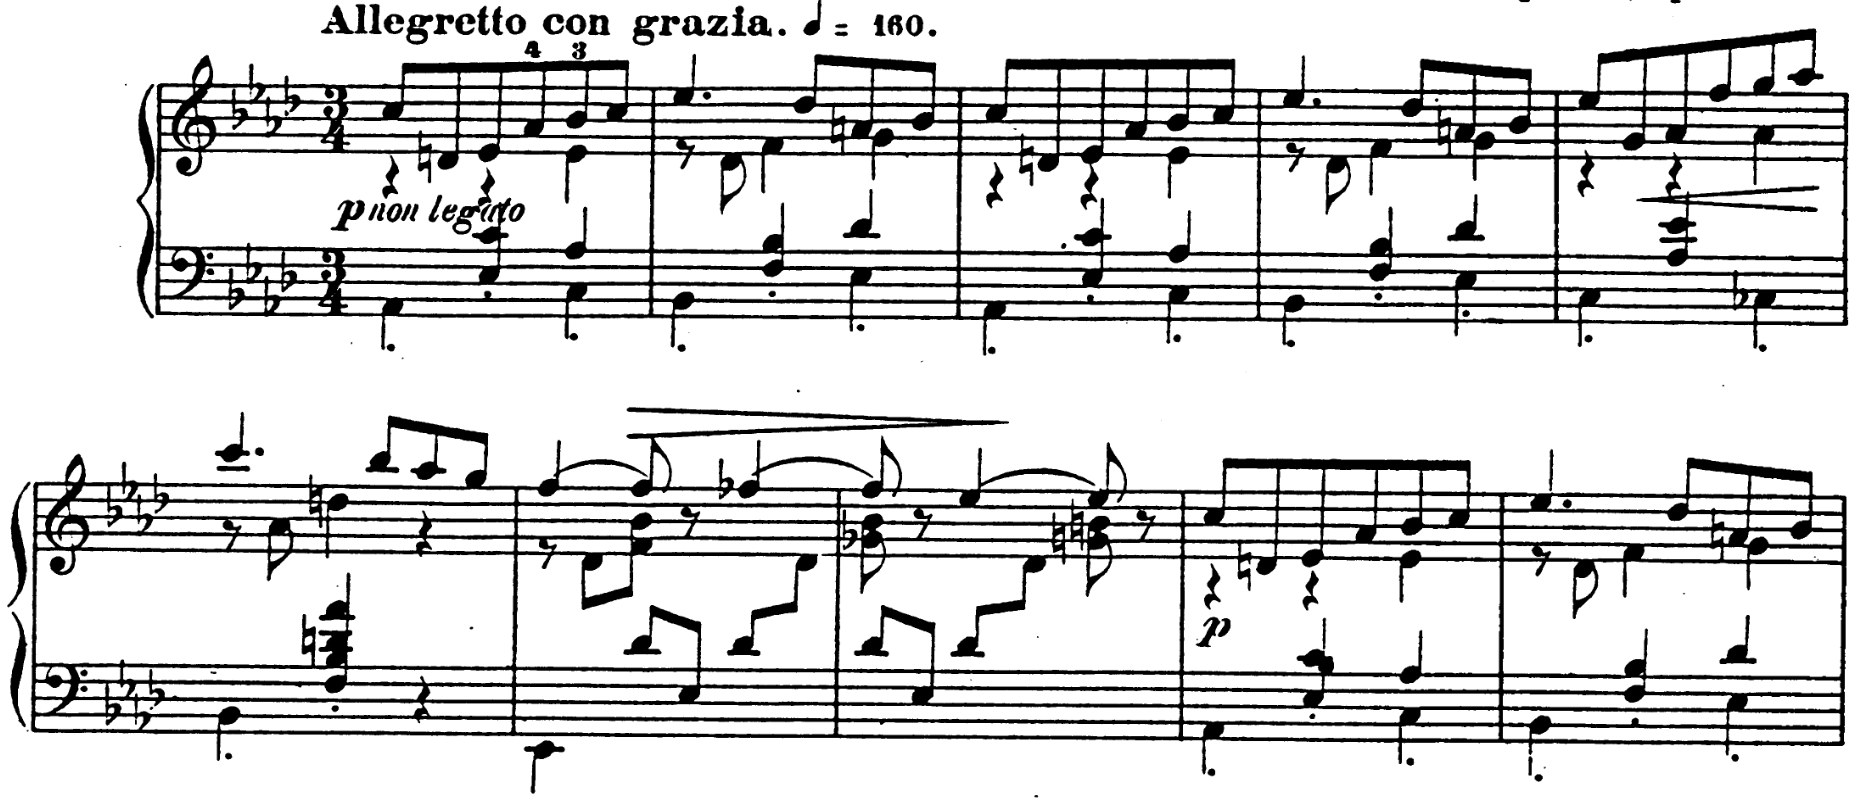
\includegraphics[width=12.5cm, keepaspectratio]{op1.png}
      &
      
\includegraphics[width=3cm, keepaspectratio]{op1-qr.png}
    \end{tabular}
  \end{bigcenter}
  \caption{\label{op1}Extrait de \emph{Trois Morceaux} op.1 \no 3 (valse).}
\end{figure}

Le nocturne op.8 (1898, voir figure \ref{op1}) est un autre hommage à Chopin. Il fait sans ambigüité référence au célèbre nocturne op.27 \no2. Toutes deux en ré$\flat$ majeur, les deux pièces partagent la même douceur et le même mystère. La mélodie, épurée mais expressive, survole un accompagnement en arpèges brisés.

\begin{figure}[!p]
  \begin{bigcenter}
    \vspace*{1.0cm}
    \begin{tabular}{lr}
      \vspace*{0.0cm}
      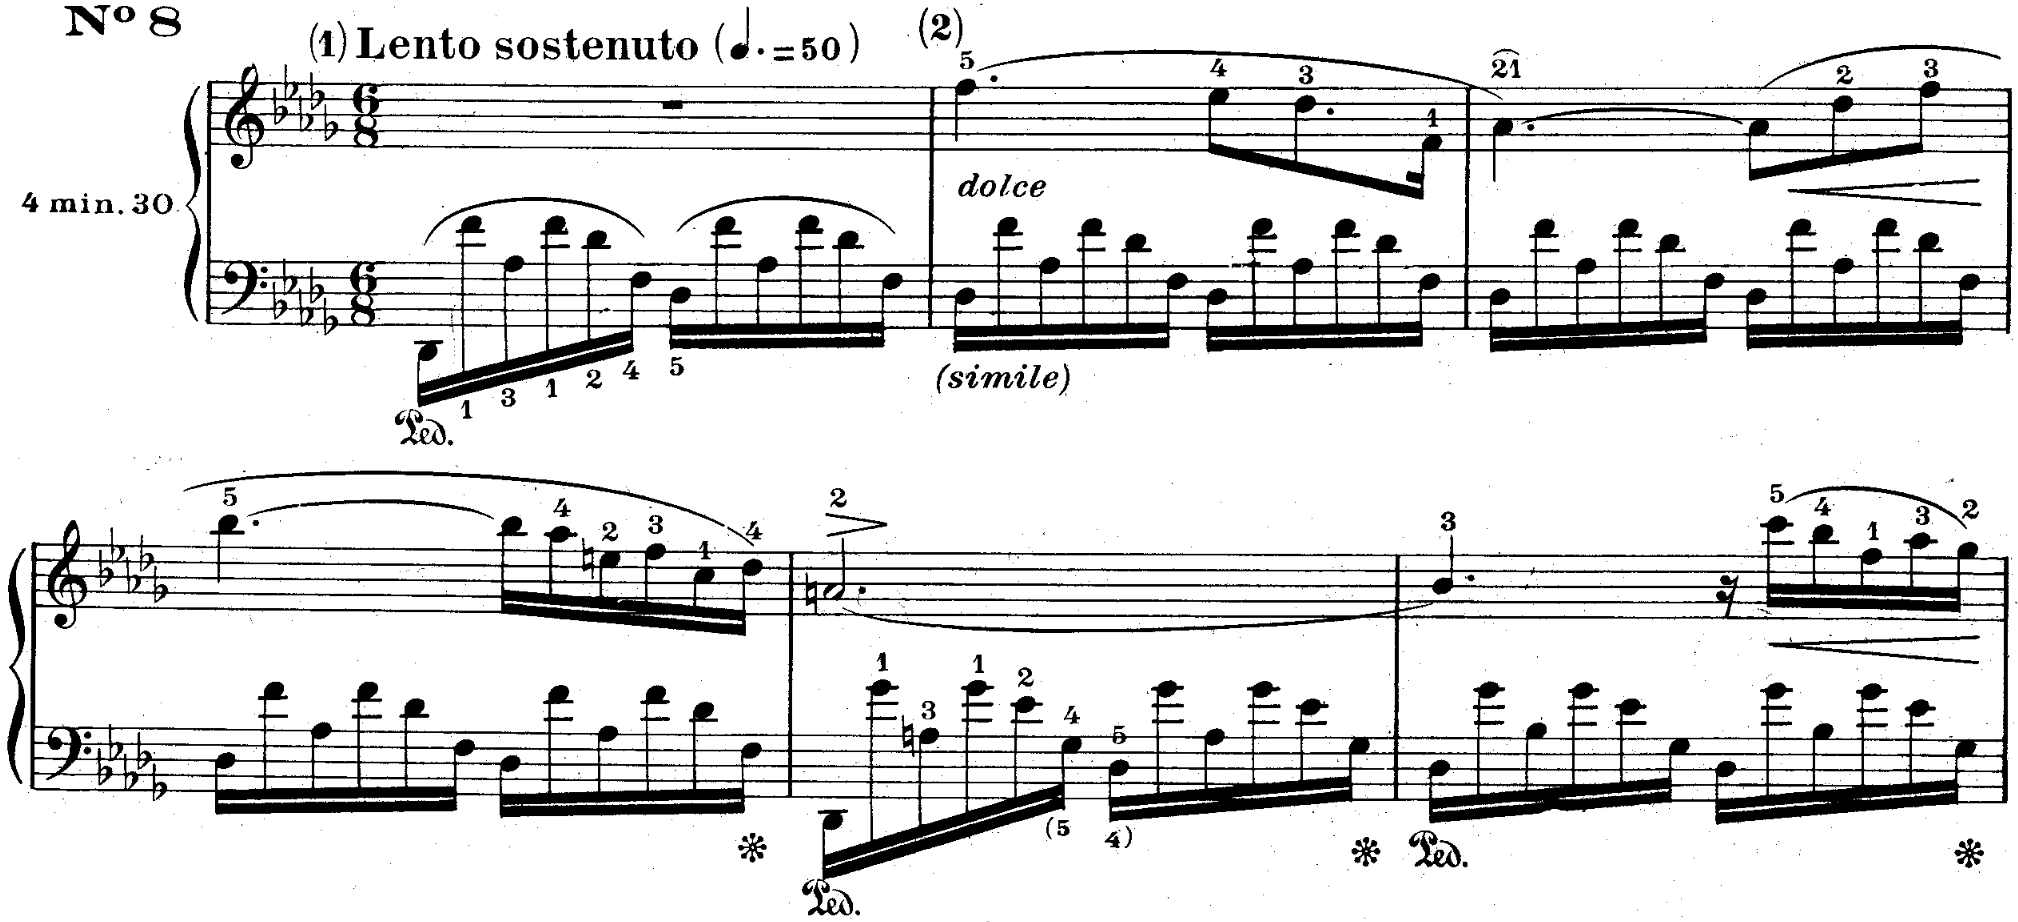
\includegraphics[width=12.5cm, keepaspectratio]{nocturne-chopin.png}
      &
      
\includegraphics[width=3cm, keepaspectratio]{nocturne-chopin-qr.png}
      \\
      \vspace{0.5cm} &
      \\
      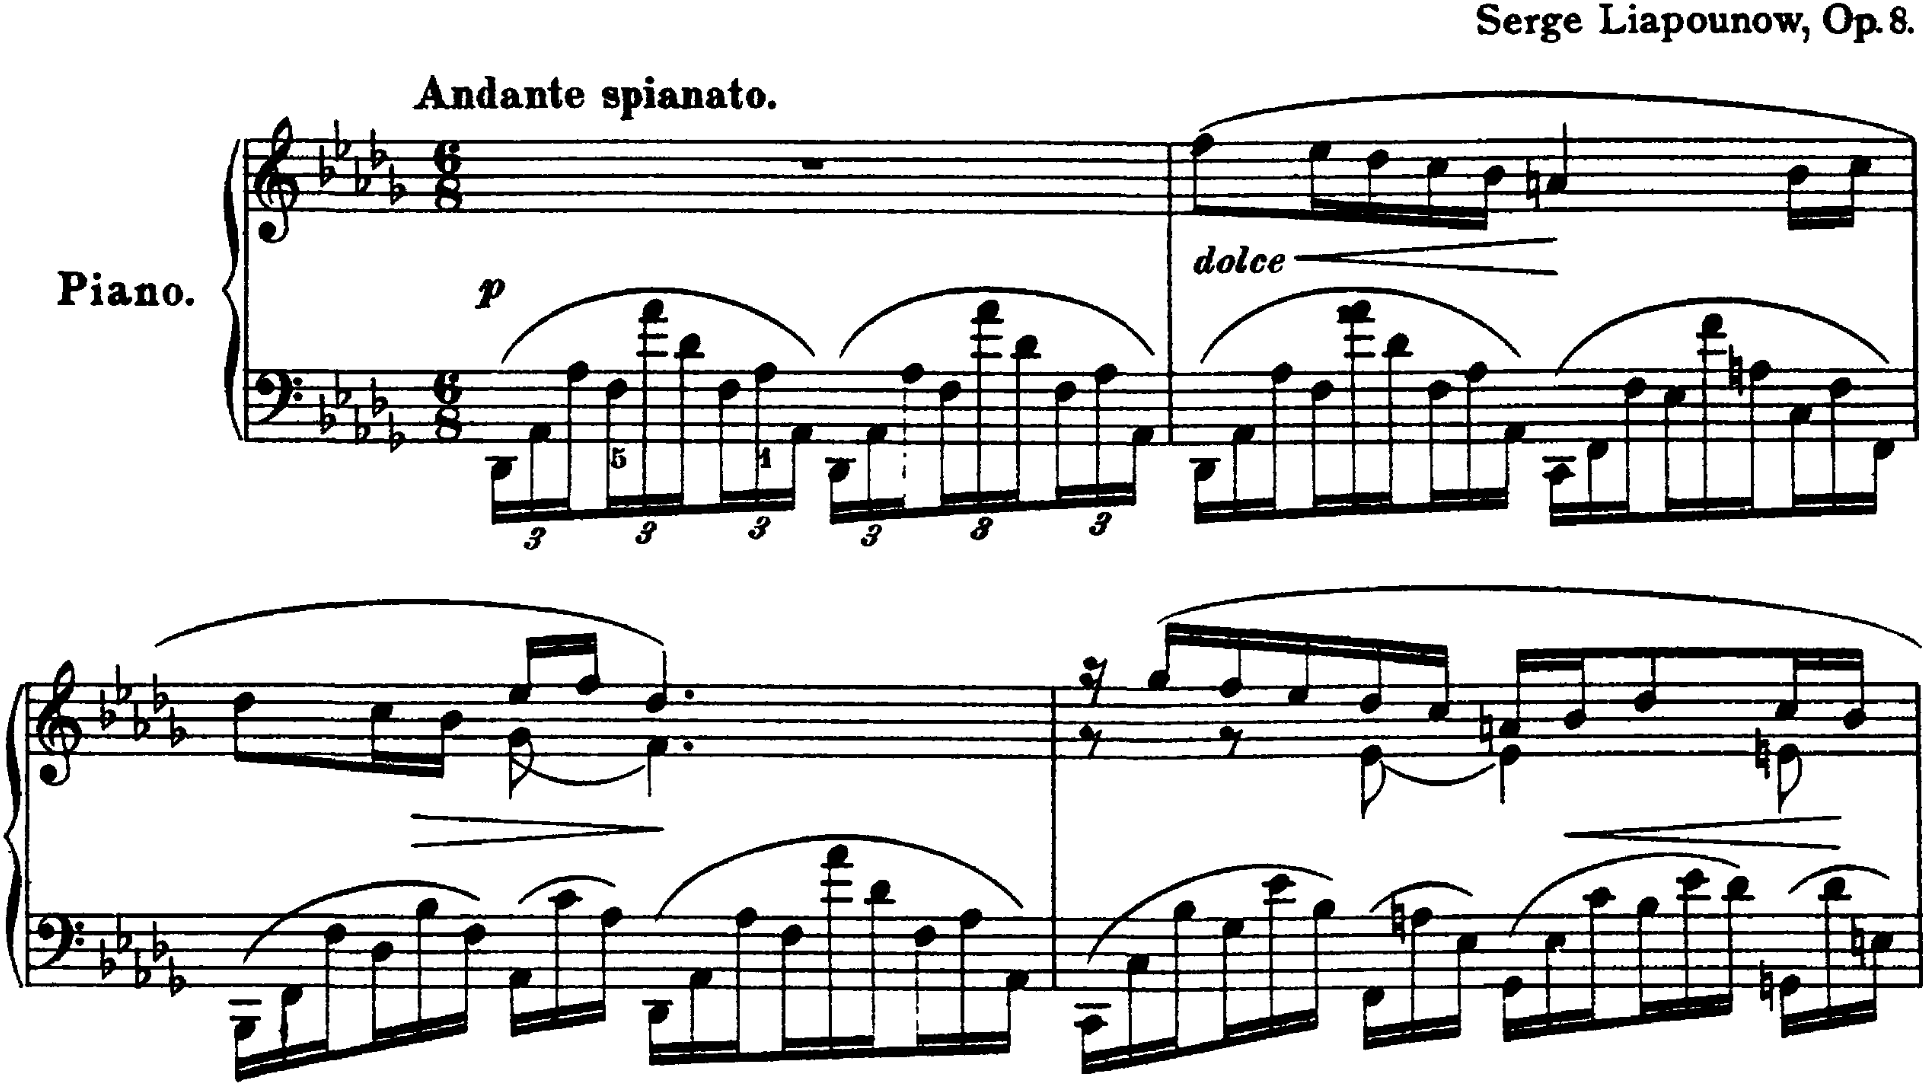
\includegraphics[width=12.5cm, keepaspectratio]{op8.png}
      &
      
\includegraphics[width=3cm, keepaspectratio]{op8-qr.png}
    \end{tabular}
  \end{bigcenter}
  \caption{\label{op11-xi}Comparaison des débuts du nocturne op.27 \no2 de Chopin (en haut) et du nocturne op.8 de Liapounov (en bas).}
\end{figure}

\newpage

La \emph{Rêverie du soir} op.3 (1880 / rev. 1903, voir figure \ref{op3}) en \emph{si} mineur est une œuvre particulièrement intéressante. Les huit premières mesures sont écrites en arpèges ascendants puis en sixtes parallèles descendantes sur une prédale de \emph{fa}$\sharp$ (dominante de \emph{si} mineur). Liapounov fait emploi d'un pentatonisme tonal aux couleurs orientales : \emph{si}, \emph{do}$\sharp$, \emph{mi}, \emph{fa}$\sharp$, \emph{sol}$\natural$ (et non sol$\sharp$). L'absence d'accord estompe la perception de la tonalité. Le rythme est d'une grande liberté et, comme le montre le grand nombre d'annotations, l'expression est recherchée. Le souffle \emph{crescendo} - \emph{decrescendo} dessine des vagues. Aux mesures 13 à 16, l'écriture en contrepoint confirme la tonalité de \emph{si} mineur avec la cadence parfaite et les harpèges de tonique mesures 17 et 18. Ces éléments sont annonciateurs du style à venir de Liapounov. La suite de l'œuvre est dans un langage plus proche du romantisme occidental. 

\begin{figure}[!h]
  \begin{bigcenter}
    \begin{tabular}{lr}
      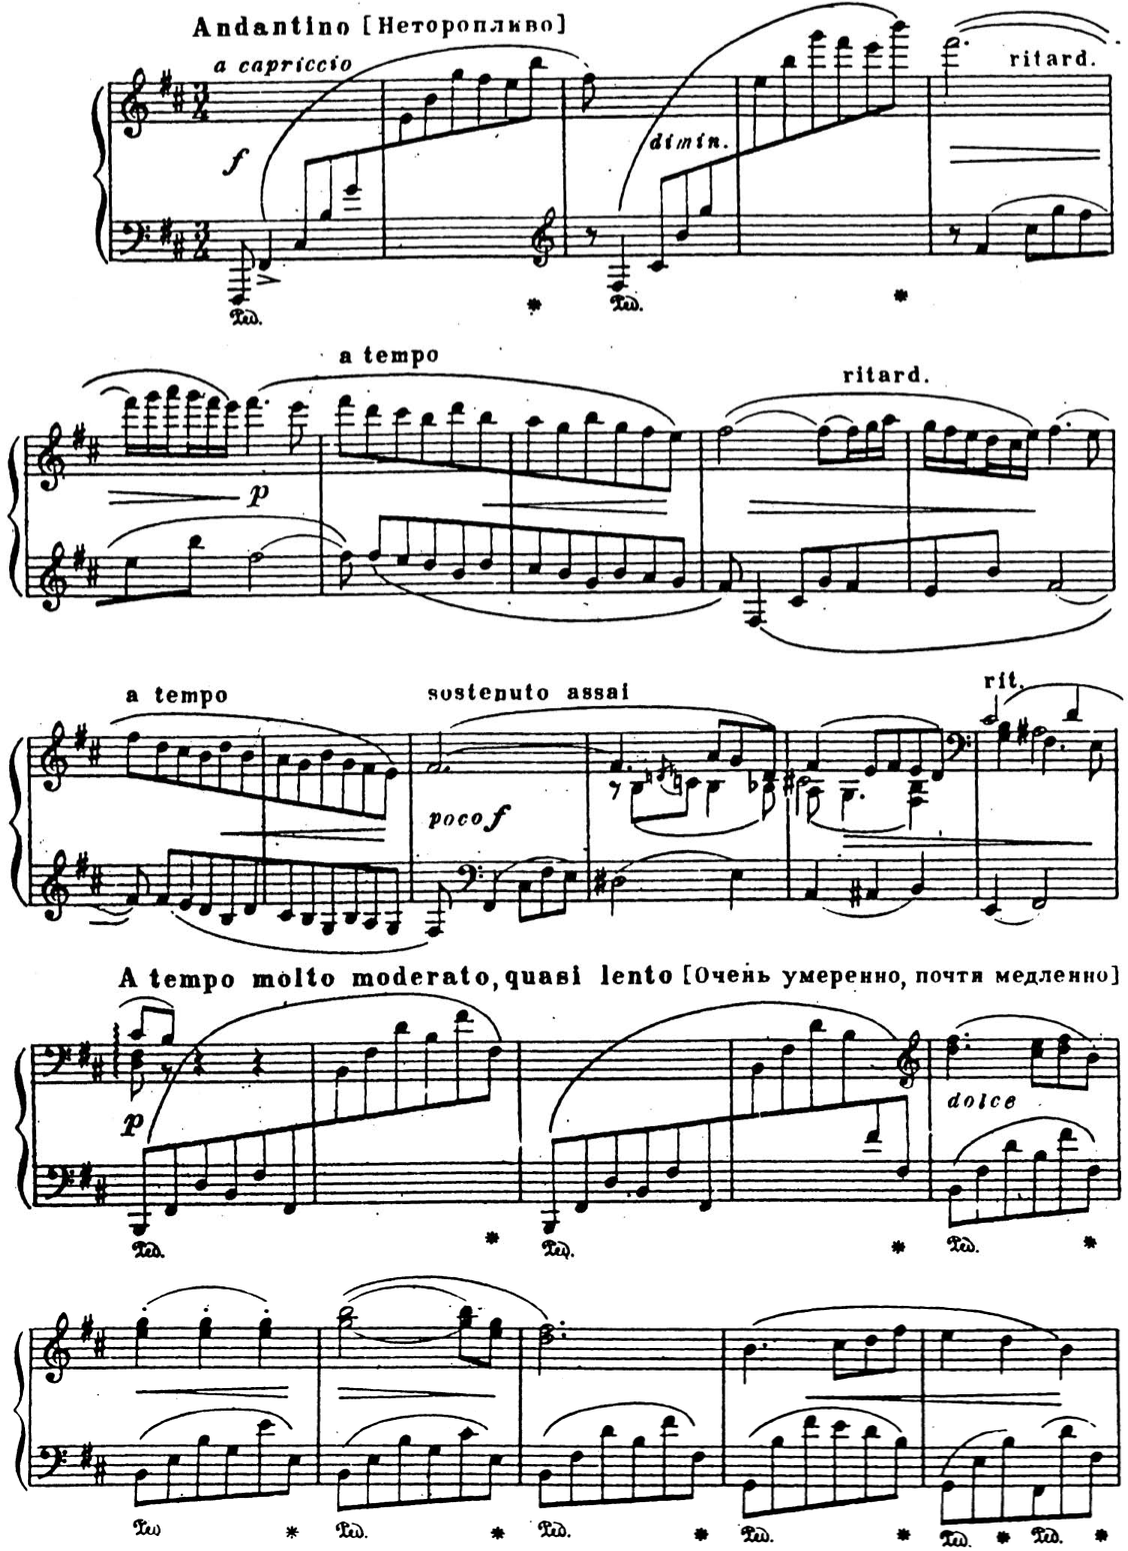
\includegraphics[width=11.25cm, keepaspectratio]{op3.png}
      &
      
\includegraphics[width=3cm, keepaspectratio]{op3-qr.png}
    \end{tabular}
  \end{bigcenter}
  \caption{\label{op3}Extrait de \emph{Rêverie du soir} op.3.}
\end{figure}

Tout au long de sa vie, Liapounov écrit des pièces aux noms évocateurs : ballades, impromptus, préludes, nocturnes, mazurkas, valses, scherzos ou autre barcarolles (voir le catalogue des œuvres annexe 1). Contrairement à Chopin, les valses et mazurkas de Liapounov sont plus développées et constituent des opus indépendants.

Cette proximité avec le répertoire des grands romantiques parisiens n'est pas du tout exceptionnelle. Elle se retrouve chez de nombreux compositeurs russes de la seconde moitié du XIX\ieme{} siècle. À titre d'exemple, le catalogue des l'œuvres de Balakirev compte de nombreuses valses, mazurkas ou nocturnes. Chez Liadov, on peut citer de cas de la valse op.9 \no 1 dont le style est presque plus chopinesque, si cela était possible, que chez Chopin lui-même (voir figure \ref{liadov}). Remarquons les nombreuses appogiatures, les sauts de registre. L'écriture de la basse est des plus simples et laisse libre cours à la mélodie.

Les compositeurs russes de la génération suivante, tels que Scriabine ou Rachmaninov, perpétueront la tradition en écrivant des recueils de préludes et d'études en hommage au génie de Chopin.\\

\vspace*{-0.25cm}

\begin{figure}[!ht]
  \begin{bigcenter}
    \begin{tabular}{lr}
      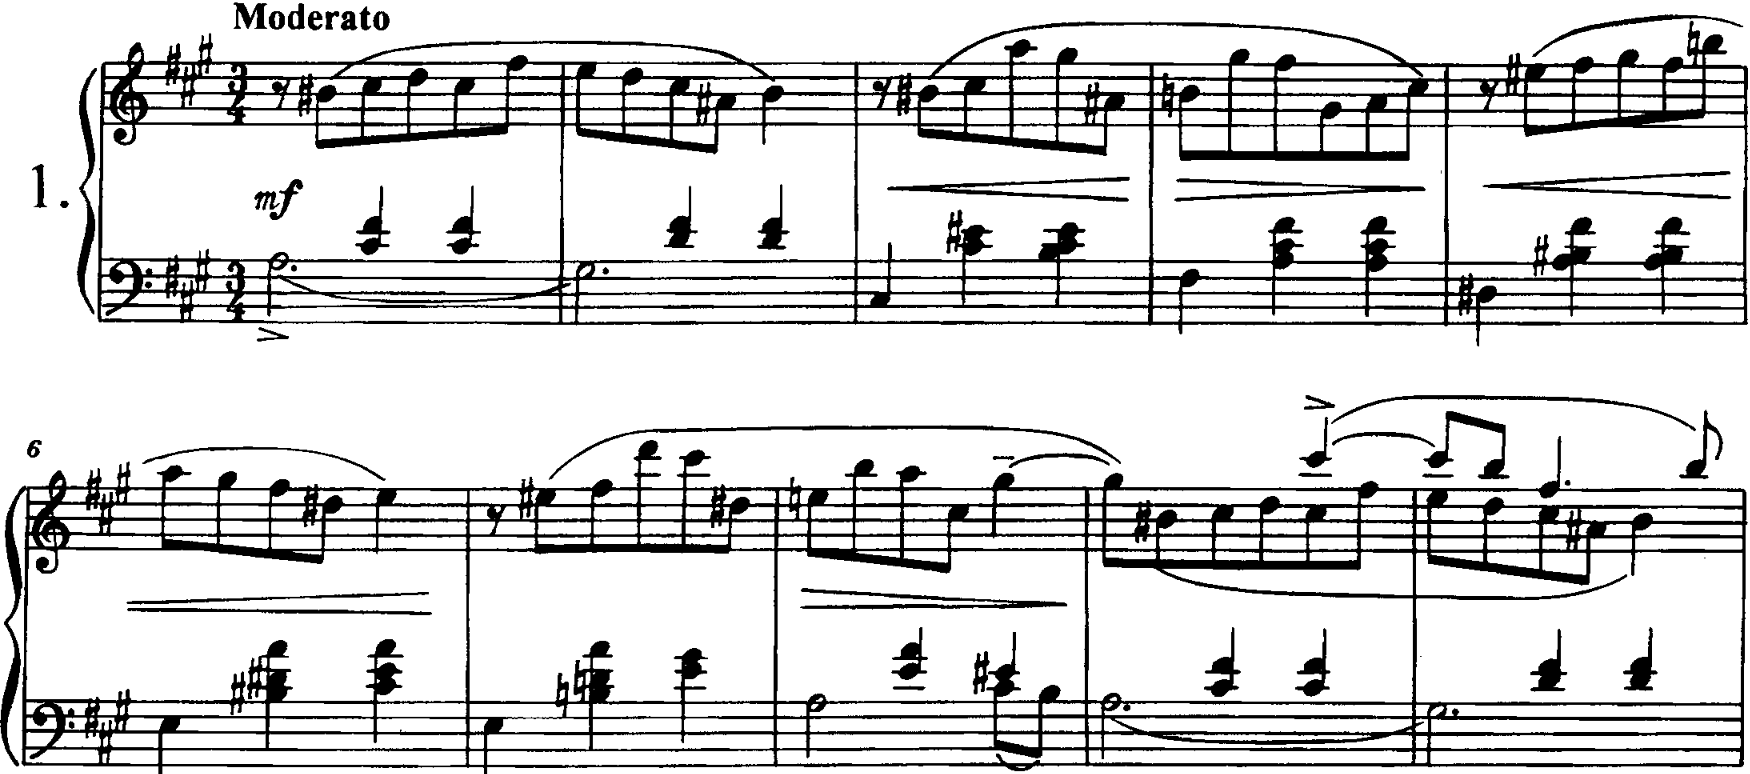
\includegraphics[width=12.5cm, keepaspectratio]{liadov.png}
      &
      
\includegraphics[width=3cm, keepaspectratio]{liadov-qr.png}
    \end{tabular}
  \end{bigcenter}
  \caption{\label{liadov}Extrait de \emph{Deux Morceaux} op.3 \no 1 (valse) de Anatoli Liadov.}
\end{figure}

\indent En 1909, lorsque Liapounov commence l'écriture de son second concerto, il écrit :\\
\indent« \emph{J'ai commencé à composer mon second concerto pour piano. [\dots] Je ne peux pas me défaire de l'influence du langage formel de Liszt. Quand il vient une écriture virtuose, je me sens complètement asservi par le pianisme lisztien.} ».\\

\vspace*{-0.25cm}

\indent Ce à quoi Balakirev répond :\\
\indent« \emph{Ne cherche pas à éviter le pianisme lisztien. Un bon compositeur ne doit pas se forcer, mais doit suivre ses tendances naturelles. [\dots] Tu ne dois pas te sentir asservi parce lorsque tu utilises le pianisme lisztien, tu peux toujours afficher ta propre personnalité.} ».

Les \emph{études d'exécution transcendante} op.11 et la sonate en \emph{fa} mineur op.27 de Liapounov sont deux magistraux hommages à Liszt. Il seront présentés dans la suite de ce mémoire. Au fil des années, c'est l'influence du \emph{Groupe des Cinq} et plus particulièrement de Balakirev qui caractérisera le style de Liapounov.

\section{L'influence de Balakirev}

À partir de 1885, Liapounov commence une association avec Balakirev qui devient à la fois son ami et son mentor. Cette relation, quasi symbiotique, durera jusqu'à la mort de Balakirev 25 ans plus tard. En 1911, Liapounov parlera en ces termes\footnote{Citation traduite du russe par Jérôme Odier.} :

« \emph{Il étonnait tout le monde par sa bravoure et par l'indépendance de sa pensée. [\dots] Il était implacable dans ses discussions, ne permettant jamais de compromis, mais en même temps, il montrait une incroyable bonté de cœur pour défendre ceux qui étaient lésés. Il ne pouvait pas supporter quelque chose de faux ou la mauvaise foi. Il a toujours été brutalement honnête et ne pouvait plier la vérité par souci de compassion. Il pouvait immédiatement rompre ses relations avec les gens qui montraient des signes d'hypocrisie ou artificialité.} »\\

Sur le plan physique, les deux hommes se ressemblent beaucoup si bien que Liapounov est parfois surnommé \emph{Balakirev le noir} en raison de la différence d'âge (22 ans) et des cheveux blancs de Balakirev.

Cette période, la plus riche pour Liapounov sur le plan musical, est de loin la moins documentée dans la littérature française et anglaise. Liapounov est le membre le plus éminent du \emph{cercle Balakirev} tardif qui succède au \emph{Groupe des Cinq}. Il est également curieux de constater le peu d'informations sur les membres de ce cerle concurant au \emph{cercle Belaïev}\footnote{Nikolai Rimski-Korsakov, Alexander Glazunov, Vladimir Stasov, Anatoly Liadov, Alexander Ossovski, Witold Maliszewski, Nikolai Tcherepnin, Nikolay Sokolov, Alexander Winkler, etc\dots} (1885-1908). Il est probable que certains compositeurs, tels que Liadov, soient passés d'un groupe à l'autre.\\

En 1887, Liapounov compose sa première symphonie sous la direction de Balakirev. Une étape importante de l'enseignement de ce dernier passe par l'écriture d'une œuvre symphonique. Liapounov se familiarise avec les éléments stylistiques de son maître ce qui influence durablement sa créativité. En 1890, il termine une de ses réalisations majeures : son premier concerto pour piano op 4 en mi$\flat$ mineur (une tonalité bien adaptée au jeu pianistique et la même que dans la première symphonie de Rimski-Korsakov). L'orchestation est très imaginative. Alors que la première symphonie peine à se faire connaitre (création en 1888, publication en 1901, rares exécutions), le concerto paraît à Berlin dès le milieu des années 1890 ce qui lui permet d'être largement mieux diffusé que des œuvres concurrentes. Il est créé le 8 avril 1891 sous la baguette de Balakirev avec l'orchestre de son \emph{école libre de musique}. C'est un vif succès et le concert « \emph{couvre plus ou moins les dépenses} ». D'autres artistes tels que Véra Scriabina (la femme d'Alexandre Scriabine à qui Liapounov dédie la très belle Barcarolle op.46) ou encore Józef Hofmann donneront le concerto à Paris et ailleurs en Russie. Précisons également qu'il remporte le prestigieux \emph{Prix Glinka Belaïev} 1904 en compagnie du concerto \no 2 de Rachmaninov. Liapounov refuse la récompense par soutient à Balakirev qui reproche à Belaïev (principal éditeur de musique russe et grand mécène, cf. \emph{cercle Belaïev}) de profiter des jeunes compositeurs pour faire grandir son influence.

\section{L'expédition de 1893}

En 1893, Liapounov est admis à la \emph{Société géographique impériale de Russie}\footnote{Elle compte parmi les plus anciennes du monde. Fondée en 1845 par le comte von Lütke, les expéditions qu'elle a organisé ont joué un rôle majeur pour la découverte et l'exploration de la Sibérie, de l'Extrême-Orient russe, de l'Asie moyenne, de l'Asie centrale ainsi que de l'océan Pacifique.}. Cette même année et accompagné de Fedore Istomin\footnote{Une gande majorité des sources biographiques stipulent, à tort, la présence de Balakirev et Liadov parmi les membres de l'expédition. Il est par contre exact que Balakirev a parcouru le Caucase et la Crimée, dès 1862, dans le même but que Liapounov 31 ans plus tard.}, il participe à une fructueuse expédition qui collecte près de 300 chansons populaires dans les régions de la Vologdan, de la Viatka et de la Kostroma. En 1894, 165 chansons sont publiées dans l'ouvrage \emph{Chansons du peuple russe} (\foreignlanguage{russian}{Песни русского народа}). Par la suite, Liapounov publie le recueil \emph{Trente chants populaires russes} op.10 puis le recueil \emph{Trente chants populaires russes} op.13. D'une longueur moyenne d'une page, chaque mélodie vient avec ses paroles et un accompagnement au piano écrit par Liapounov (voir figure \ref{chanson}). Notons qu'à ce jour, il ne semble malheureusement pas exister d'enregistrement.\\

Cette expédition marque durablement Liapounov et lui fournit une inépuisable réserve de matériaux. Comme c'est le cas dans l'étude op.11 \no 8 (voir chapitre suivant), il réutilise certains thèmes dans ses compositions. Dans le catalogue des œuvre de Liapounov (voir annexe 1), nous comptons 14 opus de chants russes\footnote{Soit 20\% des œuvres.} avec accompagnement au piano.

\begin{figure}[!p]
  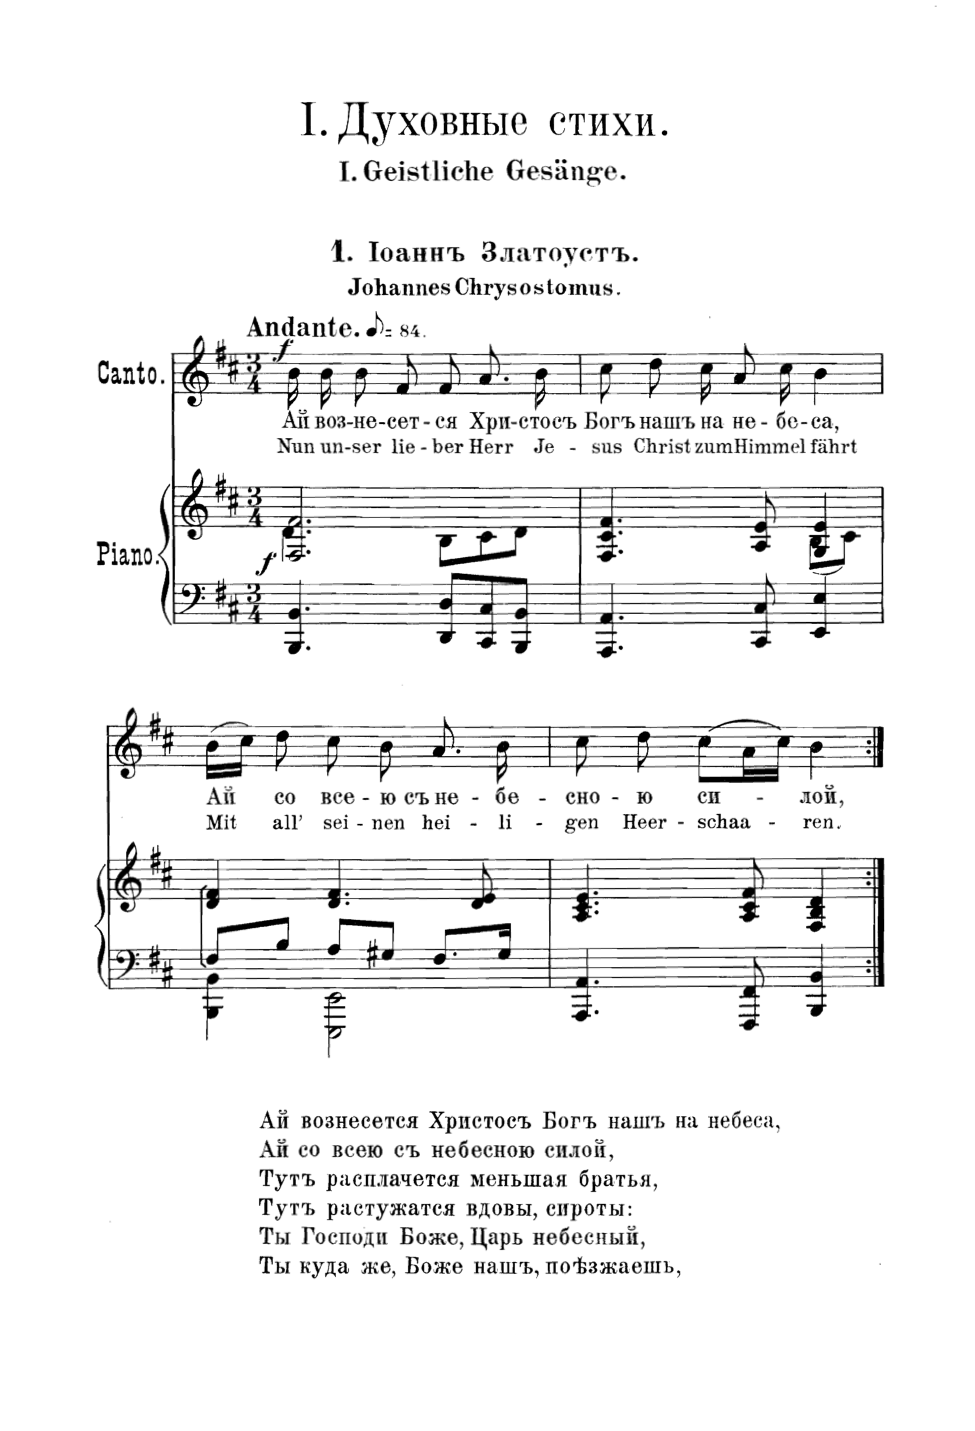
\includegraphics[width=16cm, keepaspectratio]{chanson.png}
  \caption{\label{chanson}\emph{Trente chants populaires russes} op.10 \no 1}
\end{figure}
\newpage

\section{Les \emph{études d'exécution transcendante}}

Composées entre 1897 et 1905, les 12 \emph{études d'exécution transcendante} op.11 de Liapounov représentent le sommet de son art. Cette œuvre reste malheureusement fort peu connue tant des interprètes que des musicophiles. Ce monumental cycle d'études, environ 130 pages, est un vibrant hommage à la troisième révision (1852) des 12 \emph{études d'exécution transcendante} de Franz Liszt (étude \no12 \emph{Élégie à Franz Liszt}) ainsi qu'à Balakirev (étude \no11 \emph{Lesghinka dans le style de Balakirev}). Concernant les tonalités, là où Liszt progresse par ton - ton relatif sur les touches blanches (do M - la m, fa M - ré m, etc\dots), Liapounov progresse sur les touches noires à partir de fa$\sharp$ M (fa$\sharp$ M, ré$\sharp$ m, etc\dots). Les études de Liapounov se présentent clairement comme un complément au couleurs slaves des études de Liszt :

« \emph{Il serait impoli pour moi [Liapounov] de mentionner dans le titre qu'elles constituent une suite aux études de Liszt parce que je suis relativement inconnu dans le monde de la musique. Cela pourrait être interprété comme de la vantardise. Il serait plus approprié de dédier mes études à Liszt [\dots]} »\\

\subsection{Similarités textuelles}

Les \emph{études d'exécution transcendante} de Liapounov présentent des similarités plus ou moins évidentes avec leurs modèles. Le cas le plus évident concerne l'étude \emph{La ronde des sylphes} (\no 11) dont le nom évoque déjà \emph{La ronde des Lutins} chez Liszt. Le parallèle avec \emph{Feux follets} (\no 5) est immédiat : même tempo, même mesure, même dynamique (\emph{Allegretto} chez Liszt, \emph{Allegretto scherzando} chez Liapounov). Les éléments thématiques ne sont qu'une paraphrase en \emph{sol} majeur de ceux de l'étude originale en \emph{si}$\flat$ majeur (voir figure \ref{op11-xi}).

\begin{figure}[!p]
  \begin{bigcenter}
    \begin{tabular}{lr}
      \vspace*{0.0cm}
      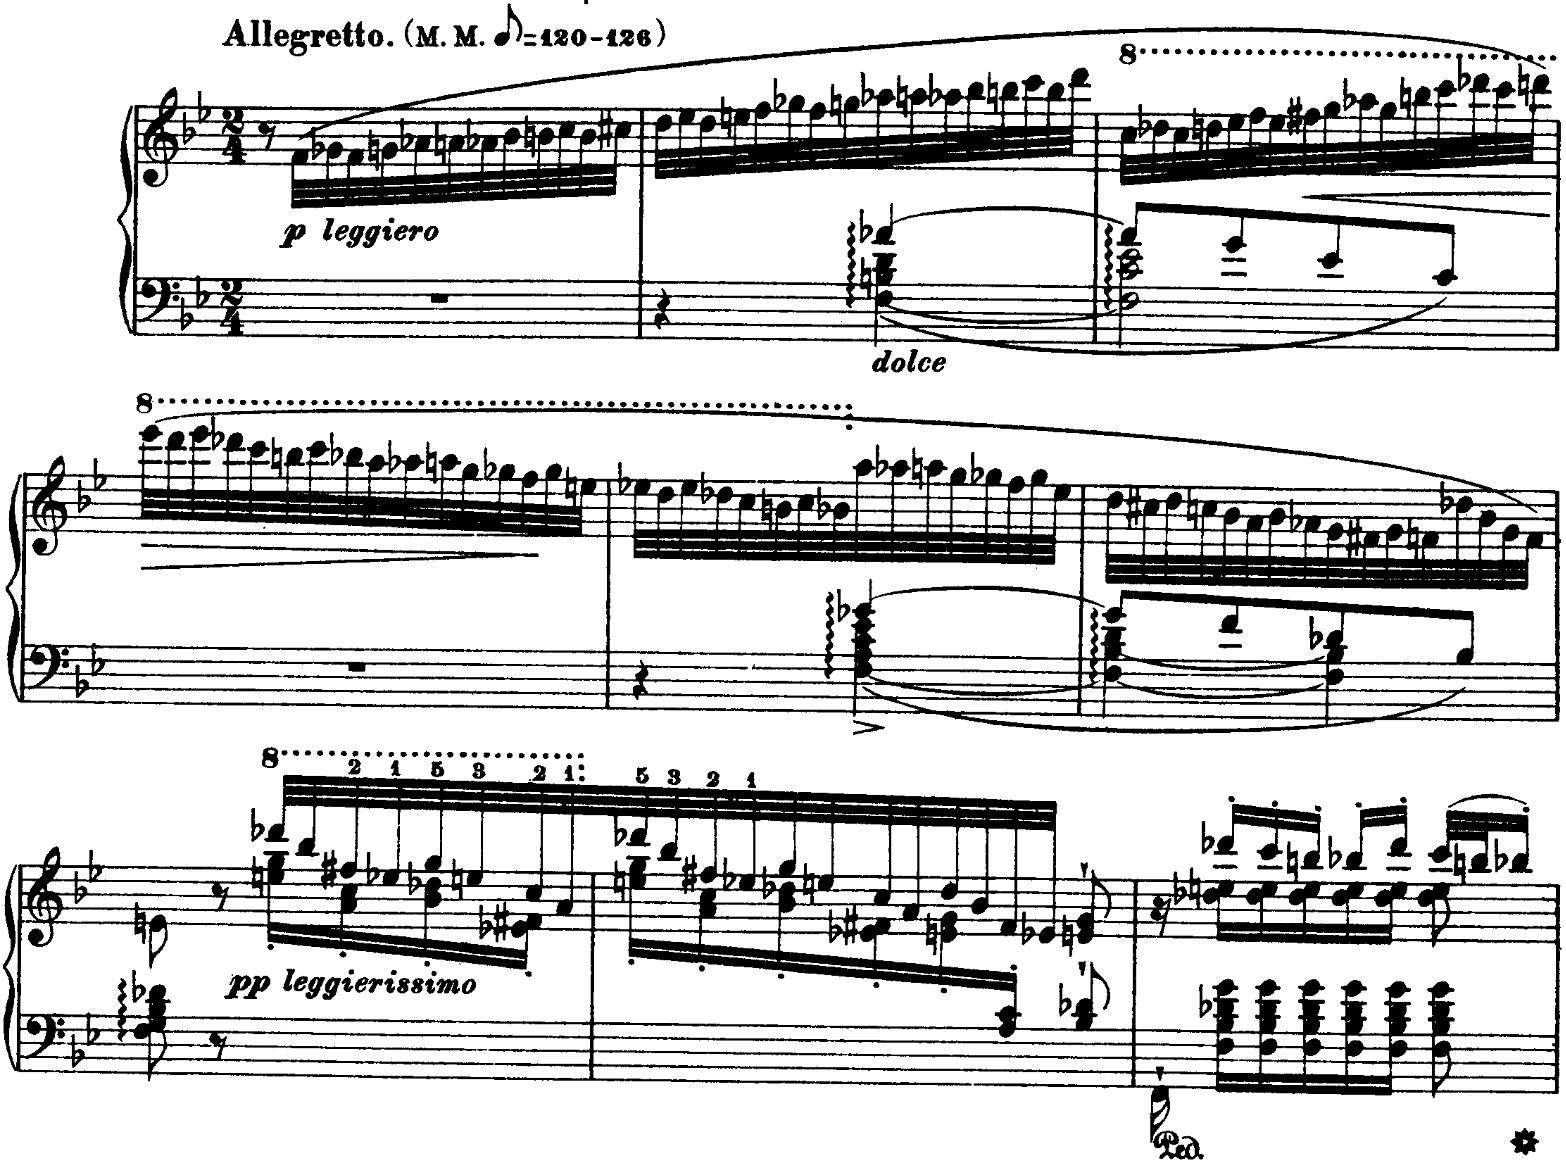
\includegraphics[width=12.5cm, keepaspectratio]{feux-follets.png}
      &
      
\includegraphics[width=3cm, keepaspectratio]{feux-follets-qr.png}
      \\
      \vspace{0.5cm} &
      \\
      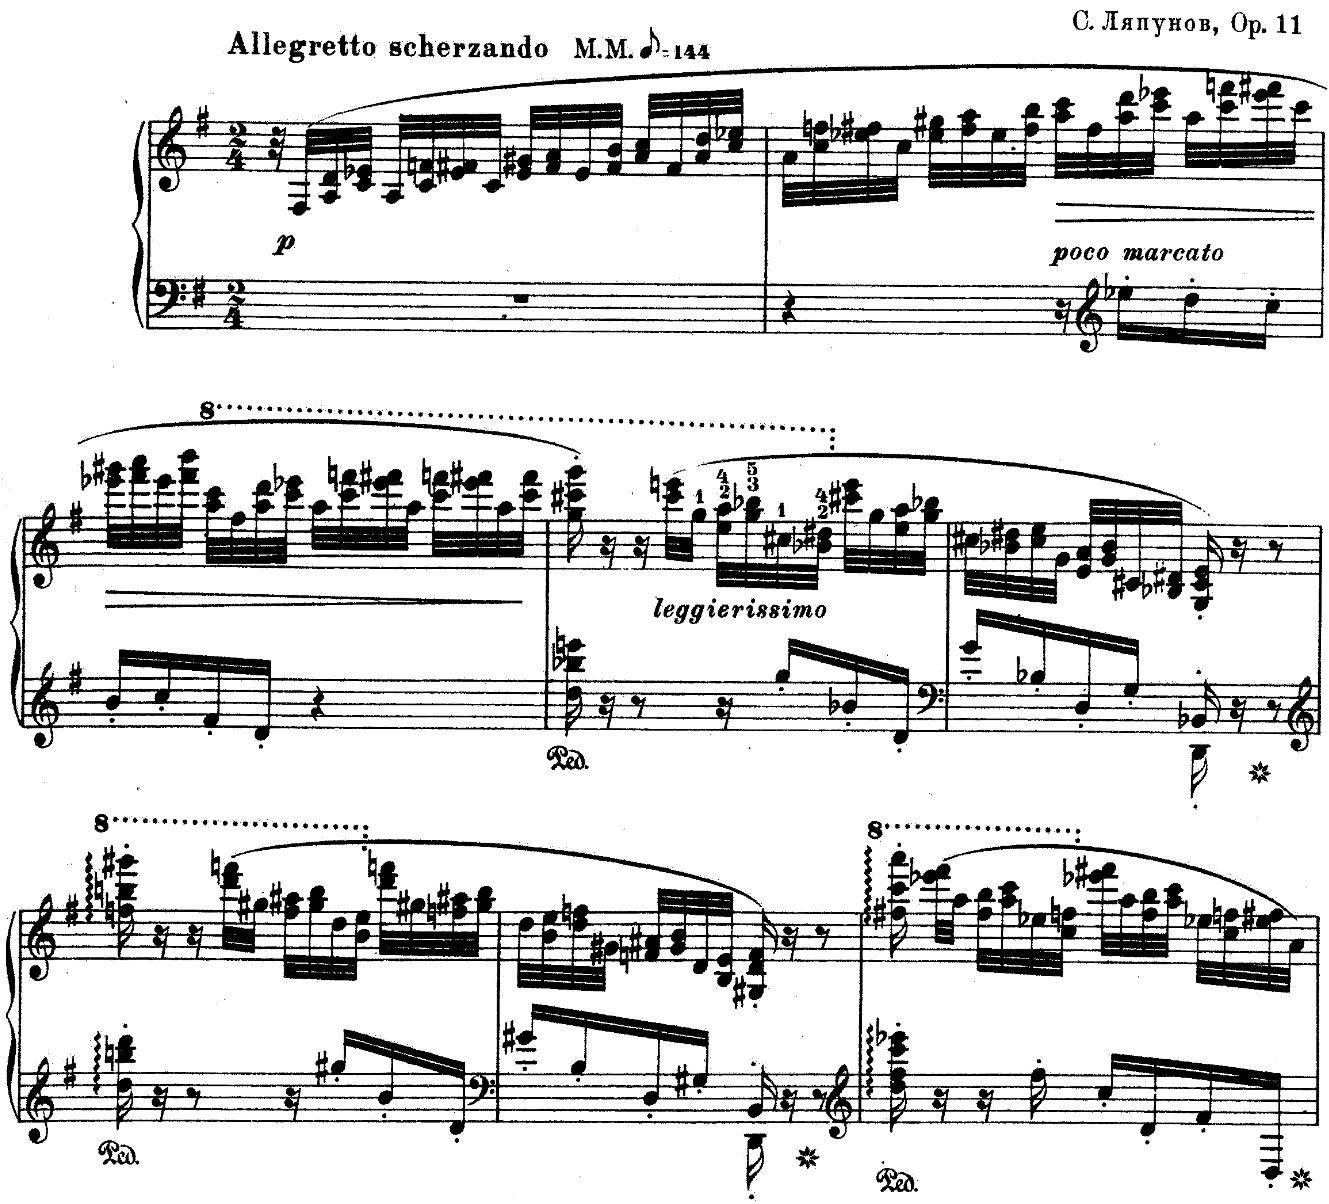
\includegraphics[width=12.5cm, keepaspectratio]{op11-xi.png}
      &
      
\includegraphics[width=3cm, keepaspectratio]{op11-xi-qr.png}
    \end{tabular}
  \end{bigcenter}
  \caption{\label{op11-xi}Comparaison des débuts de \emph{Feux follets} S.139 de Liszt (en haut) et de \emph{La ronde des sylphes} op.57 de Liapounov (en bas).}
\end{figure}

De façon similaire, il est visuellement/textuellement évident d'associer \emph{Carillon} (\no 3) et \emph{Harmonie du soir} (écriture en choral, registre médium, cloches) ainsi que \emph{Harpes éoliennes} (\no 9) et \emph{Chasse neige} (\no 12) (mesure ternaire et trémolos). De plus, il est légitime de rapprocher \emph{Nuit d'été} (\no 5) et \emph{Ricordanza} (\no 9), \emph{Tempête} (\no 6) et l'étude en \emph{fa} mineur (\no 10), \emph{Idylle} (\no 7) et \emph{Paysage} (\no 3) et \emph{Chant épique} (\no 8) et \emph{Eroica} (\no 7).\\

Avec sa pédale de fa$\sharp$ majeur et sa douce mélodie, l'étude \emph{Berceuse} (\no1) fait référence à la \emph{Berceuse} op.57 de Chopin (voir figure \ref{op11-i}). Il s'agit d'un Andantino à 4/2 de forme \emph{introduction} \emph{A=(ab)} \emph{A'=(a'b')}. L’atmosphère évoque un nocturne mais le thème est d'inspiration russe. Notons la couleur particulière des quatres premières mesures qui se construisent à partir de l'accord \emph{do}$\sharp$ \emph{sol}$\sharp$ \emph{ré}$\natural$ \emph{fa}$\sharp$ \emph{si}$\natural$ se résolvant sur \emph{do}$\sharp$ \emph{sol}$\sharp$ \emph{do}$\sharp$ \emph{mi}$\sharp$ \emph{si}$\natural$. La quarte \emph{fa}$\sharp$ \emph{si} est mise en valeur par le quart de soupir. Signalons aussi la poximité entre \emph{ré}$\natural$ et \emph{ré}$\sharp$. À partir de la mesure 8, la main gauche, en harpèges ascendants descendants, accompagne le premier thème lui-même souligné par le contre-chant de la main droite.

\begin{figure}[!p]
  \begin{bigcenter}
    \begin{tabular}{lr}
      \vspace*{0.0cm}
      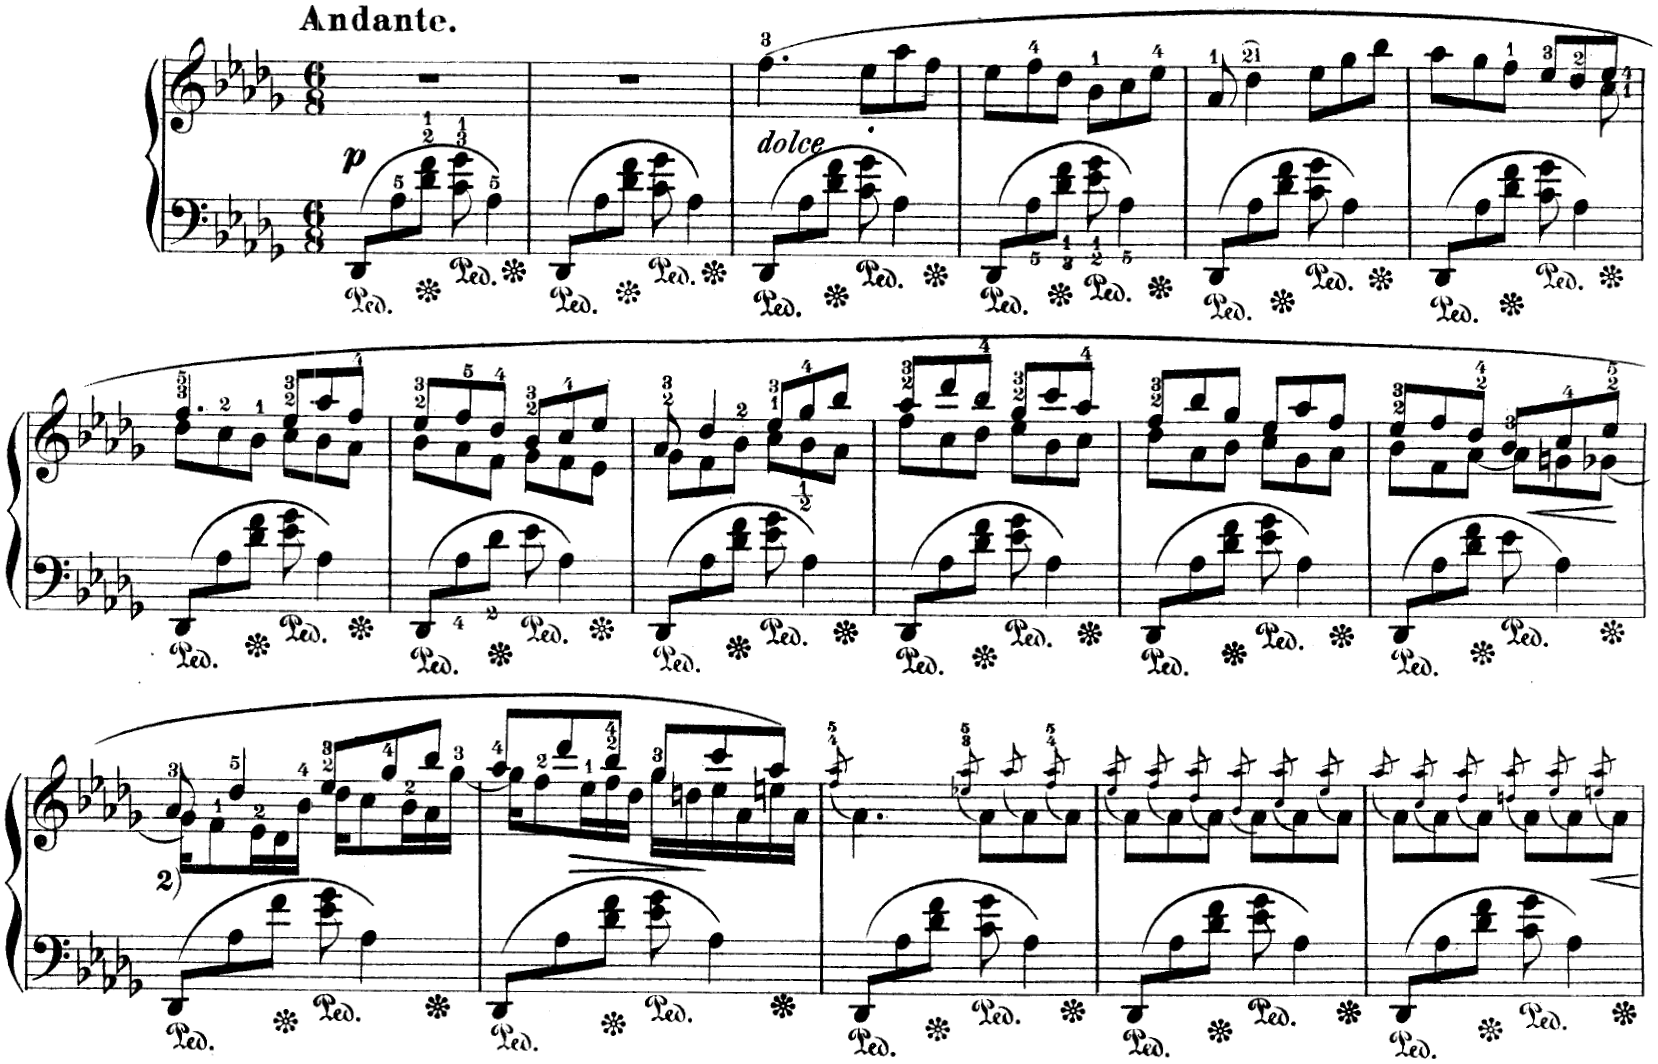
\includegraphics[width=12.5cm, keepaspectratio]{berceuse.png}
      &
      
\includegraphics[width=3cm, keepaspectratio]{berceuse-qr.png}
      \\
      \vspace{0.5cm} &
      \\
      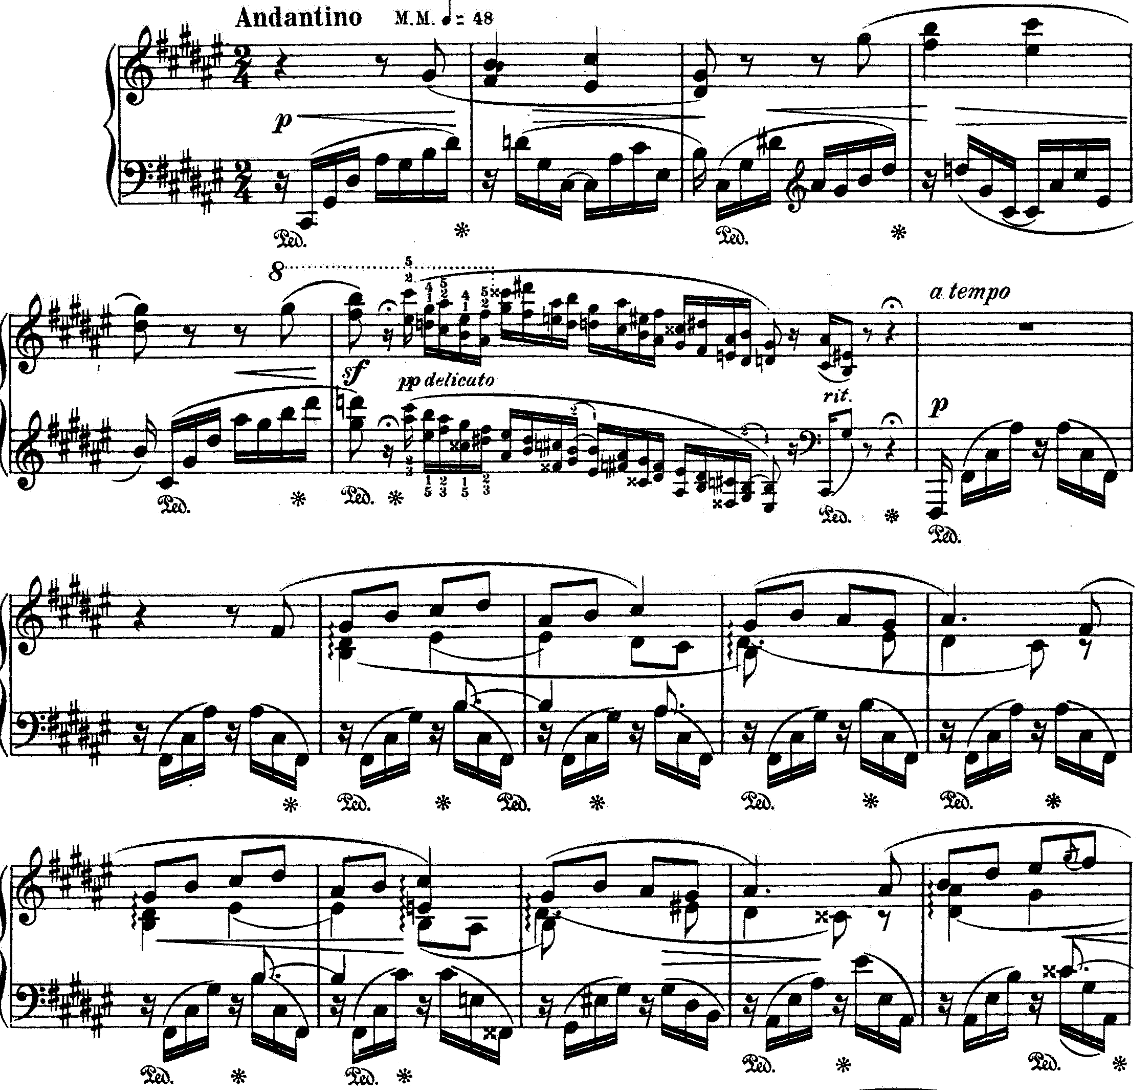
\includegraphics[width=12.5cm, keepaspectratio]{op11-i.png}
      &
      
\includegraphics[width=3cm, keepaspectratio]{op11-qr.png}
    \end{tabular}
  \end{bigcenter}
  \caption{\label{op11-i}Comparaison des débuts de la \emph{Berceuse} de Chopin op.57 (en haut) et de la \emph{Berceuse} op.11 de Liapounov (en bas).}
\end{figure}

\newpage

\subsection{Une musique à programme}

Il existe un autre point commun entre Liapounov et Liszt, leur intéret pour la musique à programme. Pour une œuvre purement instrumentale, le \emph{programme} consiste en l'ajout d'un texte d'intention par lequel le compositeur explicite ses thèmes d'inspiration afin de « \emph{préserver son œuvre de l'arbitraire d'une explication poétique erronée et d'orienter par avance l'attention sur l'idée poétique du tout ou sur un point particulier} » (notion inventée par Liszt).

Chacune des études de Liapounov dispose d'un titre en français, deux (\emph{Carillon} et \emph{Térek}) sont accompagnées d'un poème et une (\emph{Chant épique}) est inspirée du chant populaire \emph{Sorti des bois, sombres bois}.

\subsubsection{Étude III \emph{Carillon} (1901)}

La troisième étude est accompagnée d'un programme descriptif écrit par Liapounov lui-même:

« \emph{On entend l'appel d'une cloche et les sons d'un chant d'église. Le son des cloches augmente et grandi graduellement; les petites cloches se réunissent à la grande et se confondent dans un carillon général. Alternativement, se font entendre les chants solennels de l'église et les sons des cloches s’unissant enfin dans un choeur imposant que couvrent les coups lours de la grande cloche.} ».\\

La première édition de l'œuvre contient la mention « \emph{Mélodie de l’église orthodoxe russe} ». Le caractère descriptif \emph{Allegro moderato e maestoso} et orchestral évoque \emph{La Grande Porte de Kiev} des \emph{Tableaux d'une exposition} de Moussorgski.

\subsubsection{Étude IV \emph{Térek} (1900)}

La quatrième étude est accompagnée d'un court poème de Mikhaïl Lermontov\footnote{Il s'agit ici d'une traduction du russe vers l'anglais réalisée par Igor Chernyshev. L'édition Zimmermann, utilisée pour ce mémoire, ne contient qu'une traduction du russe vers l'allemand.} :

\begin{tabular}{ll}
\hspace{-3.9mm}« Térek moans, wild and wicked,
&
Scattering through the plains,
\\
Among steep mountains,
&
He appears cunning,
\\
Like a cry of a storm,
&
And in sweet adulation,
\\
Whose tears are airborne.
&
Murmurs at the Caspian Sea. »
\end{tabular}.\\

Cette étude est un double portait. Le Terek\footnote{D'une longueur de 623 kilomètres, il coule sur les territoires de la Géorgie et de la Russie et se jette dans la mer Caspienne.}, un des principaux fleuves du Caucase, est dépeint de façon violente, agitée et sauvage alors que l'utilisation d'un thème des \emph{Danses polovtsiennes} de l'opéra \emph{Le Prince Igor} de Borodine évoque la tranquillité de la mer Caspienne  (voir figure \ref{op11-iv}). Notons que l'intrigue du célèbre poème symphonique \emph{Tamara} de Balakirev, inspiré d'un poème de Lermontov, se déroule également sur les bords du fleuve Térek. Cette étude est un hommage de Liapounov au \emph{Groupe des Cinq}.

\begin{figure}[!p]
  \begin{bigcenter}
    \begin{tabular}{lr}
      \vspace*{0.0cm}
      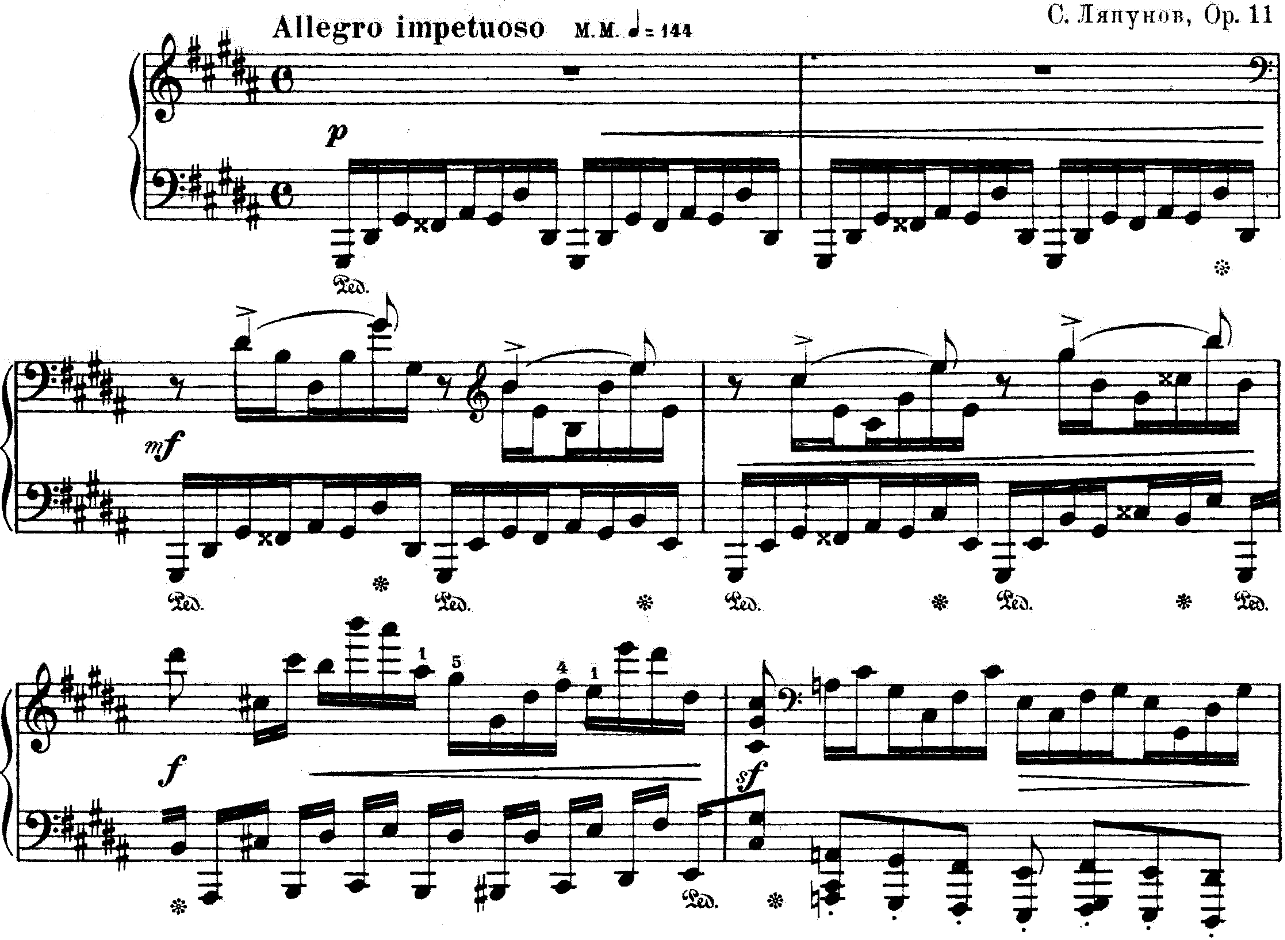
\includegraphics[width=12.5cm, keepaspectratio]{op-11-iv-1.png}
      &
      
\includegraphics[width=3cm, keepaspectratio]{op-11-iv-qr.png}
      \\
      \vspace{0.5cm} &
      \\
      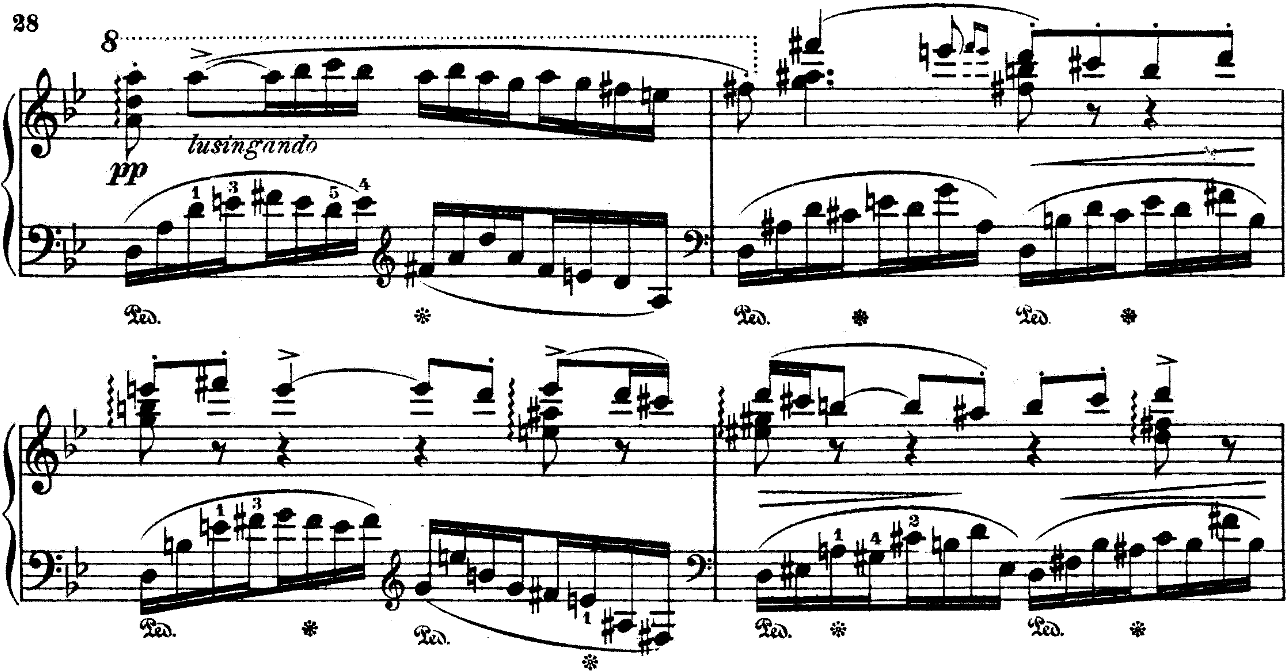
\includegraphics[width=12.5cm, keepaspectratio]{op-11-iv-2.png}
      &
      
\includegraphics[width=3cm, keepaspectratio]{op-11-iv-qr.png}
    \end{tabular}
  \end{bigcenter}
  \caption{\label{op11-iv}Début de \emph{Térek} (en haut) et citation des \emph{Danses polovtsiennes} de l'opéra \emph{Le Prince Igor} de Borodine (en bas).}
\end{figure}

\subsubsection{VIII \emph{Chant épique} (1903)}

La huitième étude s'impire du chant populaire \foreignlanguage{russian}{Из за лесу-ту, да лесу \hbox{темнова}} (\emph{Iz-za lesu, lesu temnogo} soit en français \emph{Sorti des bois, sombres bois}), collecté lors de l'expédition de 1893 et publié dans l'ouvrage \emph{Songs of the Russian People} (voir figure \ref{woods}) :\\

\begin{tabular}{ll}
\hspace{-3.9mm}« Out of the woods
&
Behind the crest
\\
  \quad{}Dark woods.
&
  \quad{}The White Tzar leads,
\\
Out of the mountain,
&
And after Himself he leads
\\
  \quad{}Steep mountain.
&
  \quad{}His mighty legions,
\\
It was not the white dawn
&
His forces,
\\
  \quad{}That appeared,
&
  \quad{}And not small ones.
\\
It was not the red sun
&
Not small forces
\\
  \quad{}That rose.
&
  \quad{}But forty-three regiments.
\\
There appeared rather
&
Forty-three regiments,
\\
  \quad{}The Tzar’s crest.
&
  \quad{}Dense with soldiers.
\\
The crest of the Tzar
&
All the soldiers
\\
  \quad{}Of the Emperor.
&
  \quad{}Who are new recruits. »
\end{tabular}\\

Il s'agit d'une \emph{byline}, une chanson narrative héroïque de la Russie ancienne. Elle dépeint une lutte épique du peuple russe contre les envahisseurs - des Mongols du Sud aux Vikings du Nord -. Dans son étude, Liapounov conserve la tonalité de fa$\sharp$ m et la signature C devient C\hspace{-2mm}|\hspace{+2mm} pour plus de dynamique. La tête du chant apparait dès la première mesure.\\

Remarque : On peut noter une certaine similarité entre le chant populaire \emph{Iz-za lesu, lesu temnogo} et le thème russe utilisé dans les \emph{Variations et Fugue sur un thème russe} op.49.

\begin{figure}[!ht]
  \begin{bigcenter}
    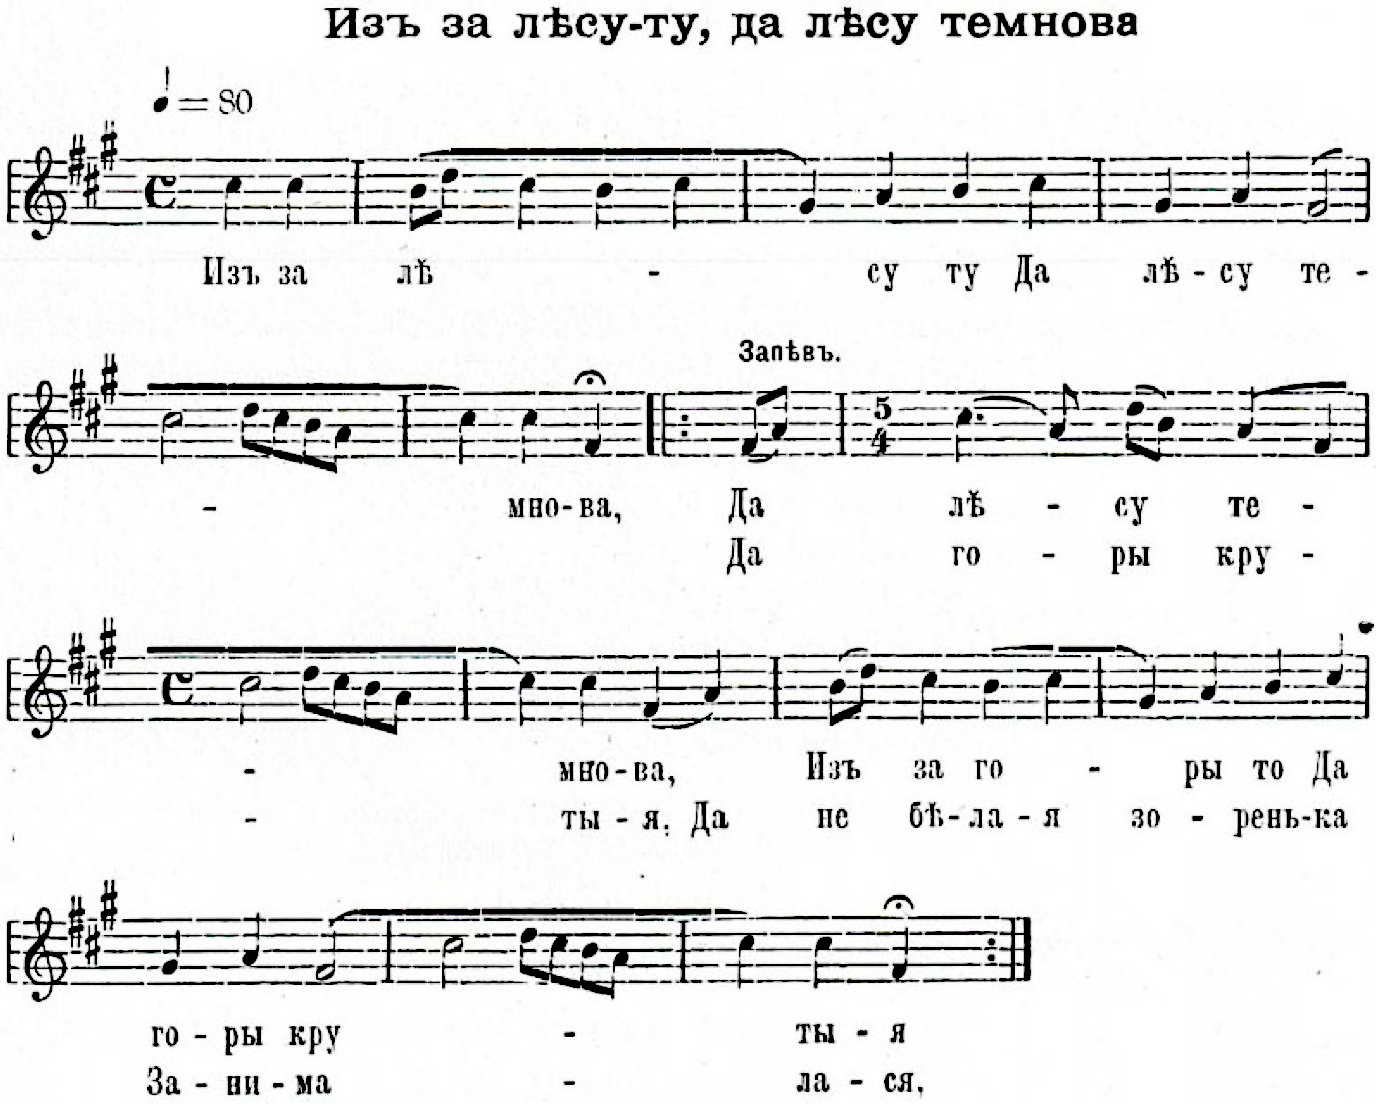
\includegraphics[width=12.75cm, keepaspectratio]{woods.png}
  \end{bigcenter}
  \caption{\label{woods}Chant populaire \foreignlanguage{russian}{Из за лесу-ту, да лесу темнова} (\emph{Sorti des bois, sombres bois}) collecté lors de l'expédition de 1893 et publié dans l'ouvrage \emph{Songs of the Russian People}.}
\end{figure}

\subsection{Sources d'inspiration russes}

L'amour de Liapounov pour les traditions anciennes (\emph{Chant épique}), l'Eglise orthodoxe (\emph{Carillon}) et la littérature russe affecte profondément le caractère de ses études. Les références et citations au \emph{Groupe des Cinq} ainsi que l'utilisation des matériaux issus de l'expédition de 1893 constellent le recueil. 

Le cas de \emph{Lesghinka} est des plus intéressants (voir partition annexe 2). De par sa qualité intrinsèque, son sous-titre « \emph{Dans le style de Balakirev} » et sa proximité avec \emph{Islamey}, la dixième étude est la plus connue du cycle. Les deux œuvres sont des danses rythmées au caractère caucasien\footnote{Une Lesghinka est une danse de la tribue des Lesghiens. Ces derniers vivent dans les montagnes du Caucase, au sud du Daghestan (Russie) et dans le nord de l'Azerbaïdjan.}, elles partagent la même signature 12/16 et sont globalement de forme \emph{A} \emph{B} \emph{A'} où \emph{B} est une partie plus calme. \emph{Lesghinka} est composée dans les tonalités préférées de Balakirev, à savoir \emph{si} mineur et \emph{ré}$\flat$ majeur.

Contrairement à \emph{Islamey}, \emph{Lesghinka} commence par une entraînante introduction de dix mesures de doubles croches annonçant le caractère général de la pièce (voir figure \ref{lesghinka-1}). La seconde augmentée \emph{ré} \emph{mi}$\sharp$ installe une couleur orientale.

\begin{figure}[!ht]
  \begin{bigcenter}
    \vspace*{0.25cm}
    \begin{tabular}{lr}
      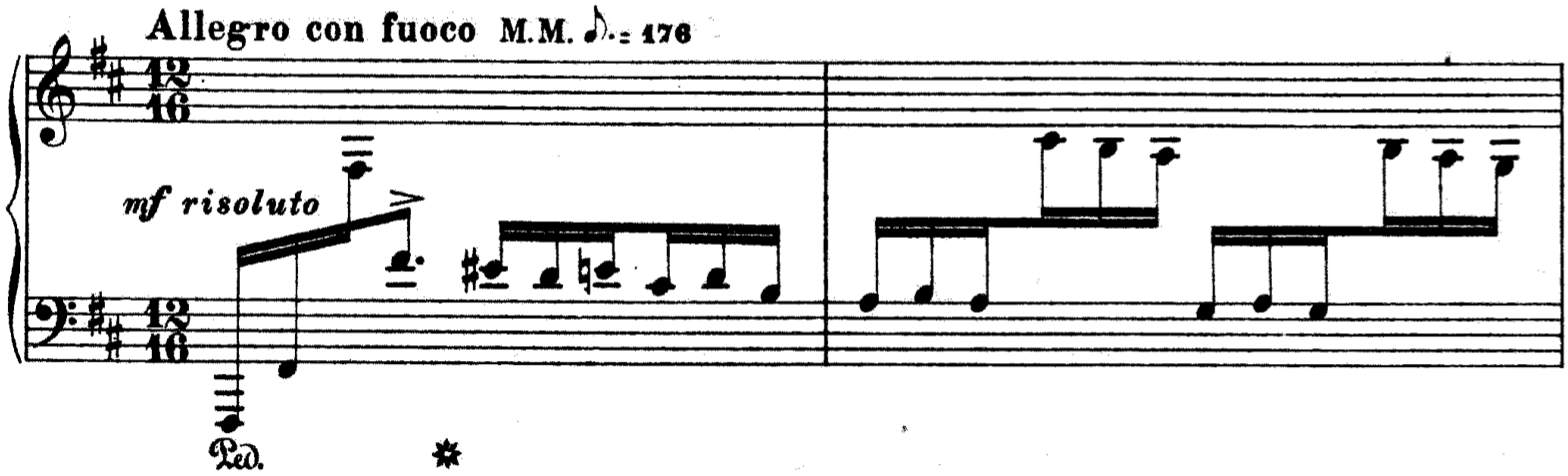
\includegraphics[width=12.5cm, keepaspectratio]{lesghinka-intro.png}
      &
      
\includegraphics[width=3cm, keepaspectratio]{op11-qr.png}
    \end{tabular}
  \end{bigcenter}
  \caption{\label{lesghinka-1}\emph{Lesghinka} (mesures 1), introduction.}
\end{figure}

L'étude est presque entièrement écrite sur pédale harpégée ce qui confère à l'œuvre un coté folklorique. Le premier thème (mesures 11, voir figure \ref{lesghinka-1}) représente un homme dansant une \emph{Lesghinka}. Notons les basses marquées, la quinte à vide de tonique, la tenue de \emph{si} à la main droite et les accents syncopés.

\begin{figure}[!ht]
  \begin{bigcenter}
    \begin{tabular}{lr}
      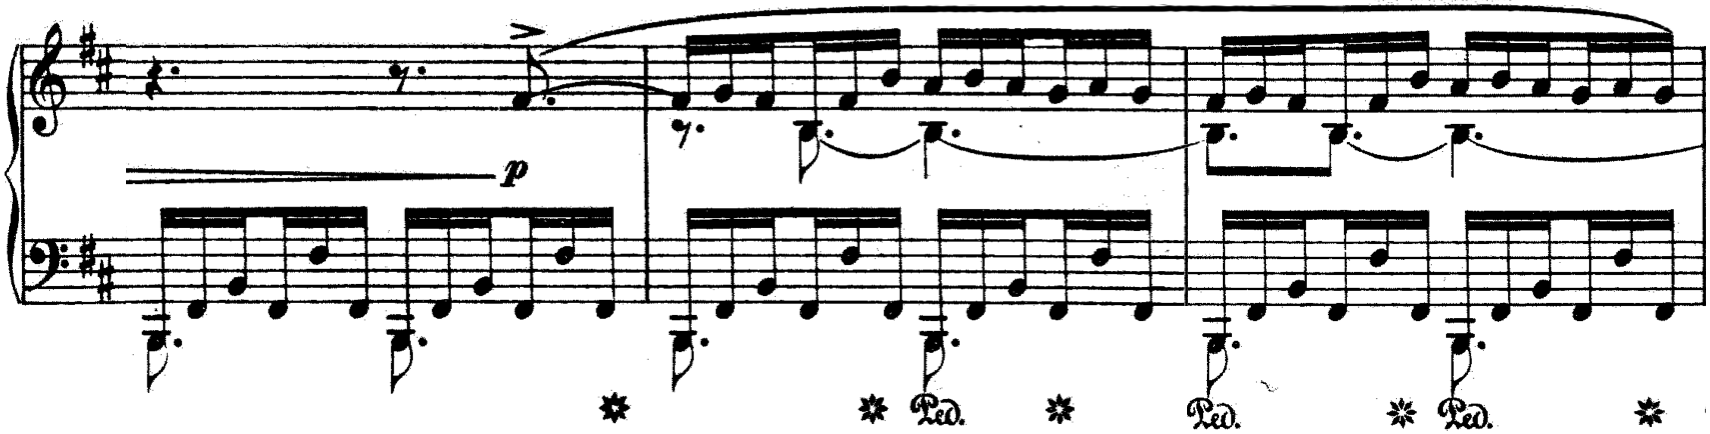
\includegraphics[width=12.5cm, keepaspectratio]{lesghinka-theme1.png}
      &
      
\includegraphics[width=3cm, keepaspectratio]{op11-qr.png}
    \end{tabular}
  \end{bigcenter}
  \caption{\label{lesghinka-1}\emph{Lesghinka} (mesure 10), premier thème.}
\end{figure}

Le deuxième thème (mesure 26, voir figure \ref{lesghinka-2} en bas) conserve le même caractère que le premier. Il commence sur prédale \emph{la} majeur et ressemble fortement au deuxième thème d'\emph{Islamey} (mesure 45, voir figure \ref{lesghinka-2} en haut).

\begin{figure}[!ht]
  \begin{bigcenter}
    \begin{tabular}{lr}
      \vspace*{0.0cm}
      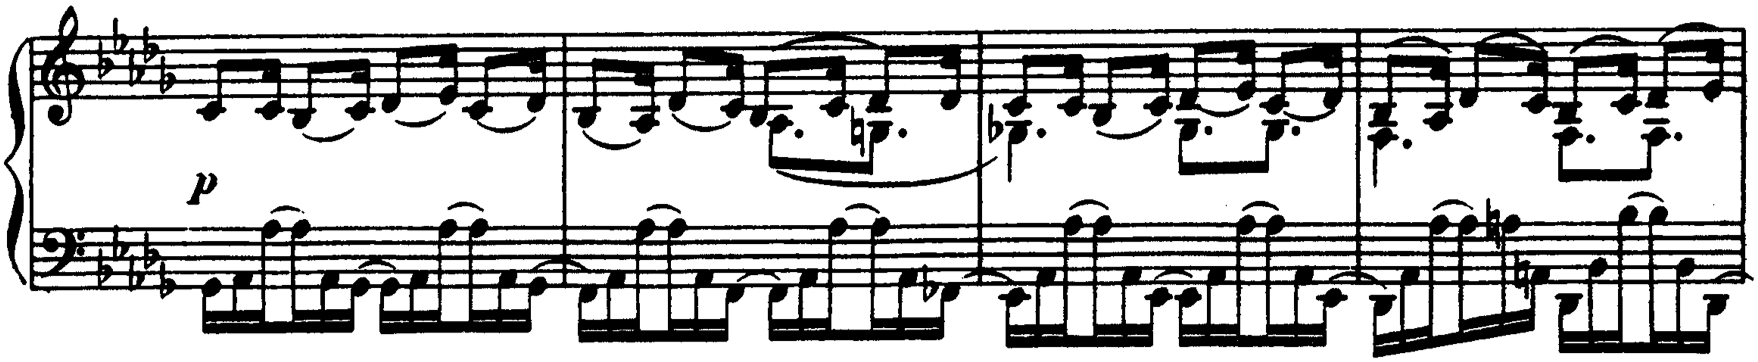
\includegraphics[width=12.5cm, keepaspectratio]{islamey.png}
      &
      
\includegraphics[width=3cm, keepaspectratio]{islamey-qr.png}
      \\
      \vspace{0.5cm} &
      \\
      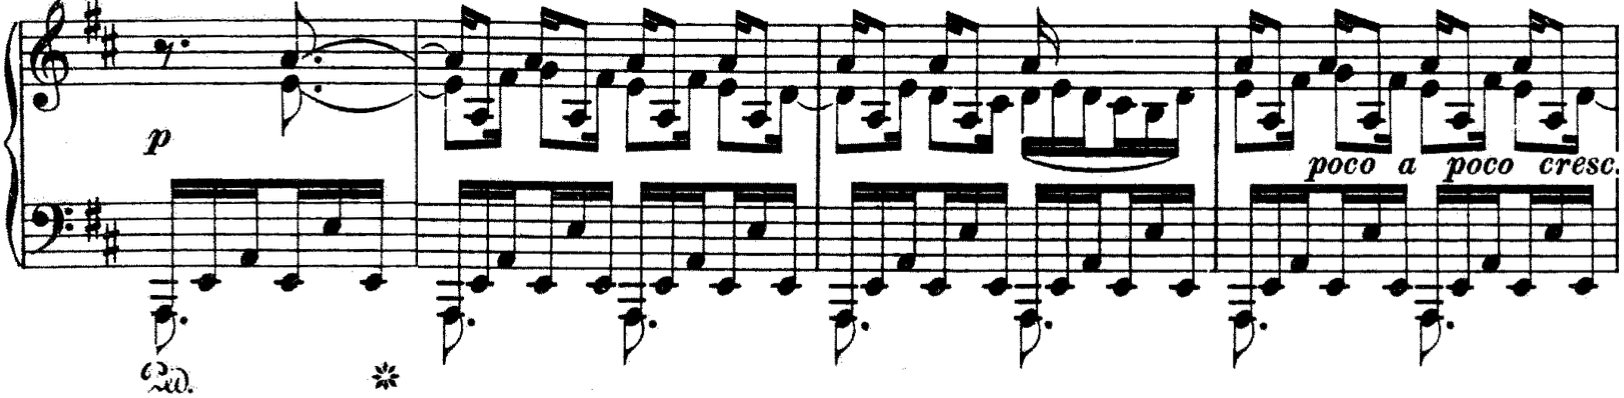
\includegraphics[width=12.5cm, keepaspectratio]{lesghinka-theme2.png}
      &
      
\includegraphics[width=3cm, keepaspectratio]{op11-qr.png}
    \end{tabular}
  \end{bigcenter}
  \caption{\label{lesghinka-2}Comparaison du deuxième thème d'\emph{Islamey} de Balakirev (mesure 45, en haut) et du deuxième thème de \emph{Lesghinka} de Liapounov (mesure 26, en bas).}
\end{figure}

Comme c'était déjà le cas pour \emph{Térek}, la partie centrale \emph{Poco pi\`{u} tranquillo} (mesure 96) est directement issue des \emph{Danses polovtsiennes} de l'opéra \emph{Le Prince Igor} de Borodine. Liapounov garde le même procédé d'écriture pianistique même si le caractère est beaucoup plus apaisé. Le contrepoint et l'harmonie sont de qualité. Remarquons la ligne descendante \emph{ré}$\flat$ \emph{do} \emph{do}$\flat$ \emph{si}$\flat\flat$ \emph{la}$\flat$ \emph{sol}$\natural$ \emph{fa} \emph{mi}$\flat$ \emph{ré}$\flat$. \\

\begin{figure}[!ht]
  \begin{bigcenter}
    \vspace*{-0.5cm}
    \begin{tabular}{lr}
      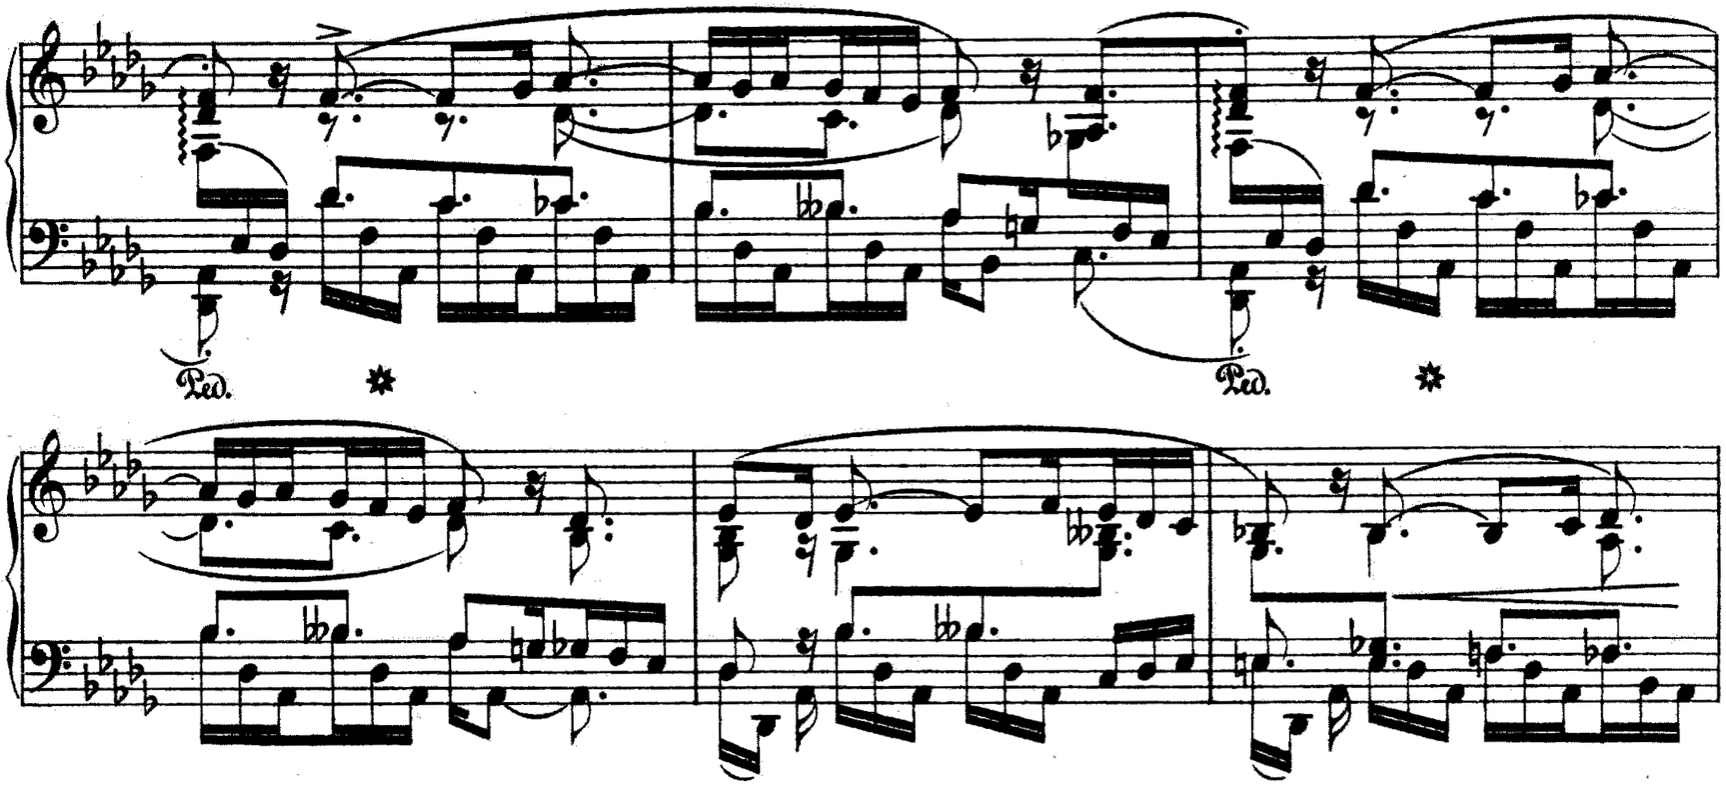
\includegraphics[width=12.5cm, keepaspectratio]{lesghinka-theme3.png}
      &
      
\includegraphics[width=3cm, keepaspectratio]{op11-qr.png}
    \end{tabular}
  \end{bigcenter}
  \caption{\label{lesghinka-3}\emph{Lesghinka} (mesures 100), thème central et citation des \emph{Danses polovtsiennes} de l’opéra \emph{Le Prince Igor} de Borodine.}
\end{figure}

Remarque : On retrouve également une lesghinka dans l'opéra \emph{Rouslan et Ludmila} de Glinka.

\subsection{L'hommage au maître}

La douzième étude \emph{Elégie en Mémoire de François Liszt}, en \emph{mi} mineur, est à la fois la dernière et la plus monumentale du recueil. Sa durée d'exécution approche les douze minutes. Elle est écrite sur le modèle des \emph{Rhapsodies hongroises} du maître auxquelles elles empreintent de nombreux éléments thématiques (en particulier à la première). La forme est libre, en un seul mouvement et, comme chez Liszt, assez proche de la fantaisie.

\subsection{Conclusion}

Au moment de sa publication en 1905, l'opus 11 de Liapounov est le plus important cycle d'études pour piano après les opus 10 et 25 de Chopin et les \emph{études d'exécution transcendante} de Liszt. Il s'agit d'un très bel hommage à ce dernier qui est aussi le dédicataire de l'œuvre. L'hommage au Groupe des Cinq, et plus particulièrement à Balakirev et Borodine (\emph{Térek} et \emph{Lesghinka}, etc\dots), est également très chaleureux.

Ces études présentent un fort intérêt pédagogique mais ne se limitent pas à la technique et à la virtuosité. Au contraire, elles re-démontrent les capacités du piano à rendre de riches couleurs orchestrales. Certaines études sont de vraies peintures sonores.

Comme le faisait Liszt, trois des études de Liapounov sont accompagnées d'éléments programmatiques. Ces derniers servent à caractériser le premier thème tandis que le(s) suivant(s) rendent compte, avec contraste, des impressions plus personnelles du compositeur.

Les très nombreuses références au folklore russe ainsi que la référence au romantisme européen positionnent ces études dans la continuité de travaux et des idéaux du \emph{Groupe des Cinq}. Même s'il demeure peu connu de nos jour, l'opus 11 constitue un sommet de la musique de Liapounov et de la musique russe.

\newpage

\section{Avant la révolution de 1917}

De 1894 à 1902, Liapounov succède à Rimsky-Korsakov comme directeur adjoint de la chapelle impériale. Après le départ de Balakirev en 1905, il est nommé directeur de l'\emph{école libre de musique} de Saint-Pétersbourg. Fondé en 1862 par Balakirev et le chef de chœur Gavril Lomakin, l'établissement propose une formation de qualité aux musiciens non professionnels.

En 1907, Liapounov effectue ses premières tournées de concerts à Berlin et Leipzig. Cette même année, il termine deux de ses œuvres majeures, sa sonate op.27 (voir chapitre 2) et sa \emph{Rhapsodie sur des thèmes ukrainiens}. Cette dernière, dédiée à Ferruccio Busoni, est un grand rondo dont le refrain \emph{Andantino pastorale}, en \emph{fa}$\sharp$, est d'une délicieuse simplicité folklorique. Deux autres thèmes servent de refrain : le bondissant \emph{Allegretto scherzando} en \emph{si}$\flat$ mineur puis l’exubérant \emph{Allegro giocoso} en \emph{fa}$\sharp$ mineur. Ce dernier est un kazachok, une danse caucasienne typiquement ukrainienne. L'œuvre se termine par une énergique coda. D'avantage que pour le premier concerto, la \emph{Rhapsodie sur des thèmes ukrainiens} requiert du pianiste une extraordinaire virtuosité lisztienne. Elle est publié par Julius Heinrich Zimmermann en 1907 et la création est assurée au printemps 1909 par l'orchestre de l'\emph{école libre de musique} et compositeur au piano.

En 1909, Liapounov compose son poème symphonique \emph{Żelazowa Wola} - le village natal de Chopin en Mazovie - pour célébrer le centenaire de la naissance du « Mozart polonais ». Le début de l'œuvre cite la célèbre mazurka en \emph{la} mineur op.17 \no 4. Une fois les commémorations passées, Liapounov s'emploie à terminer une autre de ses œuvres majeures, son second concerto pour piano. L'introduction orchestrale est un véritable chef-d'œuvre du répertoire romantique du genre. Le premier thème \emph{Lento ma non troppo}, en \emph{mi} majeur, évoque l'univers imaginaire, exotique et oriental de la première symphonie en \emph{ut} majeur de Balakirev. Les deux concertos apportent une réelle contribution à la littérature romantique pour piano et gagneraient à être d'avantage connus.

En 1910, Liapounov est chargé de compléter les œuvres inachevées de Balakirev. C'est ainsi qu'il termine le concerto en \emph{mi}$\flat$ majeur op. posthume (1861-1862 puis 1906-1910) d'une manière vraisemblablement approuvée par son mentor, qu'il réalise une orchestration d'\emph{Islamey}\footnote{En plus de l'orchestration de Sergueï Liapounov (1914), il existe une seconde orchestration, moins populaire et techniquement moins abordable, réalisée par Alfredo Casella (1908).} et qu'il transcrit quelques pièces orchestrales pour piano à quatre mains. Âgé de 73 ans, Balakirev meurt le 29 mai 1910 à Saint-Pétersbourg.\\

À partir de 1910, Liapounov devient professeur de piano, d'histoire de la musique et de composition au conservatoire de Moscou. Dans sa classe de piano, il ne prend que des élèves avancés. Son enseignement s'adapte spécifiquement à chaque situation et se concentre essentiellement sur l'interprétation et l'utilisation « juste » du rubato.

\newpage

En 1914-1915, Liapounov écrit encore quelques-unes de ses plus belles pages de musique avec ses \emph{Variations sur un thème géorgien} op.60 où l'on retrouve tout l'univers sonore des \emph{Danses polovtsiennes} ou du poème symphonique \emph{Dans les steppes de l'Asie centrale} de Borodine. En 1915, il termine son Concerto pour violon et orchestre en \emph{ré} mineur op.60 et son sextuor pour piano, deux violons, alto, violoncelle et contrebasse en \emph{si}$\flat$ mineur op.63.\\

\section{Après la révolution de 1917}

De 1916 à 1923, Liapounov connait une grave crise créative. En 1917 seulement, il termine sa seconde symphonie commencée sept années auparavant. Du fait de la révolution, les conditions de vie deviennent très difficiles. Le conservatoire de Moscou fonctionne au ralenti et les spectacles sont complètement interrompus. Dans ses lettres, Liapounov se plaint de sa mauvaise santé, de la faim, du froid et son incapacité à jouer du piano et composer. C'est dans cette période que naît l'idée d'émigrer à l'étranger. Cependant, cette perspective implique la séparation avec tout ce qui lui est cher, la Russie d'un part, et surtout sa famille. Au début des années 1920, le compositeur est dans un état voisin du dèsespoir. À son frère Boris, il écrit :\\
« \emph{[\dots] Vivre au jour le jour devient insupportable [\dots] », « [\dots] Je pense que le voyage serait nécessaire pour moi, si je dois encore travailler [\dots]} ».\\

Un événement précipite le départ. En mars 1922, au cours d'une opération de saisie des biens de l'Église, Liapounov refuse de cèder les clefs de la chapelle du conservatoire de Pétrograd (Saint-Pétersbourg). Il est traduit en justice et, à l'issue du procès, est condamné à six mois de d'emprisonnement. Au plus bas moralement et physiquement, il se résout à partir.\\

Liapounov s'installe à Paris dès 1923. Il reprend très vite ses activités de concert. Au cours de la saison 1923-1924, il interprète ses pièces pour piano solo, son sextet, sa seconde symphonie et des ballades orchestrales arrangées pour deux pianos avec le pianiste Maurice Dumesnil (un élève de Claude Debussy). Le 31 octobre 1924, Liapounov participe à l'inauguration du conservatoire folklorique russe de Paris. Pour l'occasion, il joue avec Prokofiev l'ouverture de l'opéra \emph{Rouslan et Ludmilla} de Glinka dans une version arrangée pour deux pianos. Il a de nombreux projets d'avenir, il dirige, entre autre, une école de musique pour émigrés russes. Pour l'automne 1924, il prépare une série de concerts mais meurt d'une attaque cardiaque quelques heures avant le premier d'entre eux, le 8 Novembre 1924, à l'âge de 64 ans.\\

Les figures \ref{liapounov1} et \ref{liapounov2} montrent quelques photographies de Sergeï Liapounov à différentes périodes de sa vie.

\begin{figure}[!p]
  \begin{bigcenter}
    \begin{tabular}{lr}
      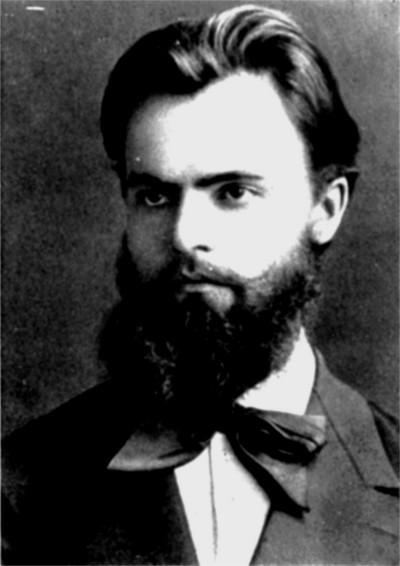
\includegraphics[width=7cm, keepaspectratio]{lyapunov-1.jpg}
      &
      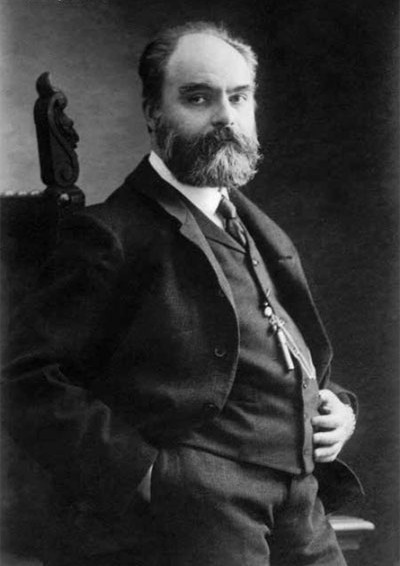
\includegraphics[width=7cm, keepaspectratio]{lyapunov-2.jpg}
    \end{tabular}
  \end{bigcenter}
  \caption{\label{liapounov1}Sergueï Mikhaïlovitch Liapounov (\foreignlanguage{russian}{Сергей Михайлович Ляпунов}).}
\end{figure}

\begin{figure}[!p]
  \begin{bigcenter}
    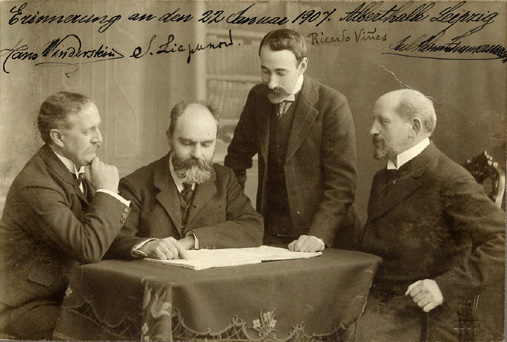
\includegraphics[width=14cm, keepaspectratio]{lyapunov-3.jpg}
  \end{bigcenter}
  \caption{\label{liapounov2}Hans Winderstein (chef d'orchestre), Sergeï Liapounov (compositeur), Ricardo Viñes (pianiste) et Julius Heinrich Zimmermann (principal éditeur de Balakirev et Liapounov) à Leipzig en 1907.}
\end{figure}

\newpage

\section{Un compositeur oublié}

Avec un catalogue de plus de 70 opus (soit un peu plus que Balakirev) comptant de grandes formes pianistiques et symphoniques (les \emph{études d'exécution transcendante}, la sonate en \emph{fa} mineur, deux symphonies, deux poèmes symphoniques, deux concertos, la \emph{Rhapsodie sur des thèmes ukrainiens}, \dots), Liapounov reste largement oublié des musicologues comme des interprètes tant en Europe qu'en Russie.

L'étude, même rapide, de son œuvre attestent pourtant de la place de choix qu'il occupe aux cotés de Balakirev dans une période de profonde mutation politique et culturelle. Sans prétendre à l'exhaustivité, essayons de dégarer quelques éléments pour comprendre cette situation :

\begin{enumerate}
  \item Liapounov est issue d'une génération intermédiaire de compositeurs dont la visibilité a peut-être été éclipsée par l'éclat du \emph{Groupe des Cinq} d'une part et par l’avant-garde russe (Scriabine, Stravinsky, Prokofiev) d'autre part.
  \item Liapounov est le dernier représentant, et sans aucun doute le plus constant, des membres des cercles de Balakirev.
  \item Liapounov est resté fidèle à l'idéal musical initié par Glinka et perpétué par le \emph{Groupe des Cinq}.
  \item La grande virtuosité de la musique de Liapounov la rend pianistiquement peu abordable.
\end{enumerate}

%%%%%%%%%%%%%%%%%%%%%%%%%%%%%%%%%%%%%%%%%%%%%%%%%%%%%%%%%%%%%%%%%%%%%%%%%%%%%

